\documentclass[11pt]{article}
\usepackage[a4paper,left=22.5mm,right=22.5mm,top=25mm,bottom=25mm]{geometry}
\usepackage[T1]{fontenc}
\usepackage[utf8]{inputenc}
\usepackage[scaled=0.92]{helvet}
\renewcommand{\familydefault}{\sfdefault}
\usepackage{amsmath,amssymb,bm}
\usepackage{graphicx}
\usepackage{float}
\usepackage[font=small,labelfont=bf,labelsep=period]{caption}
\graphicspath{{figures/}{./}}

\renewcommand{\figurename}{Supplementary Fig.}
\renewcommand{\thefigure}{S\arabic{figure}}
\renewcommand{\theequation}{S\arabic{equation}}
\newcounter{suppnote}
\newcommand{\suppnote}[1]{\refstepcounter{suppnote}\section*{Supplementary Note \arabic{suppnote}: #1}}
\newcommand{\blurb}[1]{\textbf{#1}}
\setlength{\parindent}{0pt}
\setlength{\parskip}{6pt}

\begin{document}

\begin{center}
{\Large\bfseries Supplementary Information}\\[4pt]
{\large A Unified Recurrent Circuit Model of Normalization and Sensory Adaptation}
\end{center}

\subsection*{Conventions used throughout}
All simulations used the configuration of the ensemble experiments of the main text: 13 principal neurons per receptive field (RF), one classical RF (cRF) and five surround RFs, a frame of $K=182$ interneurons per RF, $\sigma=0.15$, $\beta=\tfrac12$, all-ones normalization weights unless stated, and a 40~ms delay of normalization signals from the surround. Stimuli were gratings at contrast $c=80\%$, presented for 32~ms each. ``Small'' stimuli covered the cRF only and ``large'' stimuli covered the cRF and the surround. Time constants were those of the simulation code ($\tau_y=0.4$, $\tau_a=0.2$, $\tau_u=30$, $\tau_v=30$, $\tau_g=500$, $\tau_\mu=2000$~ms), which differ from the table in the Methods of the main text. In the biased ensemble one orientation (the adaptor) made up 38\% of presentations. Unless stated, the circuit adapted for 4~s starting from zero gains. Before any experiment we confirmed that simulated steady states matched Eqs.~10 and 11 of the main text (relative error below $10^{-9}$ for zero gains and below $10^{-6}$ for adapted gains with non-negative $\bm{z}'$) and that halving the time step changed adapted gains by less than $10^{-5}$.

Two readouts were used. \emph{Frozen-gain readout (small adaptors):} gains were frozen at the end of adaptation and steady-state responses to large test gratings were computed. \emph{In-stream readout (large adaptors):} responses were read at the last time step of each presentation during adaptation, as in Section~2.3 of the main text. The \emph{suppression profile} is each neuron's peak response after adaptation to the biased ensemble divided by its peak response after adaptation to the uniform ensemble (1 means no change), plotted against the neuron's preferred orientation relative to the adaptor. Gains were active during adaptation to both ensembles.

%=====================================================================
\suppnote{Revised circuit equations}

The simulations in this Supplement used the following form of the circuit equations:
\begin{align}
\tau_y \frac{d\bm{y}}{dt} &= -\bm{y} + \beta\,\bm{z} + \left(\frac{1}{1+\bm{a}^+}\right)\bm{W}_{yy}\sqrt{\bm{y}^+} - \bm{u}^+ \odot \bm{W}_{yv}\bm{v} \label{eq:dy}\\
\tau_u \frac{d\bm{u}}{dt} &= -\bm{u} + \left(\frac{\sigma}{2}\right)^2 + \bm{N}\left(\bm{y}^+ \odot {\bm{u}^+}^2\right) \label{eq:du}\\
\tau_a \frac{d\bm{a}}{dt} &= -\bm{a} + \bm{u}^+ + \bm{a}\odot\bm{u}^+ \label{eq:da}\\
\tau_v \frac{d\bm{v}}{dt} &= -\bm{v} + \bm{g}\odot\bm{c}, \qquad \bm{c} = \bm{W}_{yv}^\top\sqrt{\bm{y}^+} \label{eq:dv}\\
\tau_g \frac{d\bm{g}}{dt} &= (\bm{c}-\bm{\mu})^2 - \bm{\theta}_t \label{eq:dg}\\
\tau_\mu \frac{d\bm{\mu}}{dt} &= -\bm{\mu} + \bm{c} \label{eq:dmu}
\end{align}
with the notation of Section~3.2 of the main text. They differ from Eqs.~4--9 of the main text in one term: the adaptive feedback is gated by the firing rate $\bm{u}^+$ of the normalization interneurons instead of $\bm{a}^+/(1+\bm{a}^+)$. At steady state Eq.~\ref{eq:da} gives $\bm{u}^+=\bm{a}/(1+\bm{a})$, so the fixed point (Eqs.~10 and 11 of the main text) is unchanged. They differ from our earlier simulation code in three ways: (i) the gate; (ii) the gain multiplies the input to $\bm{v}$ (Eq.~\ref{eq:dv}) rather than the feedback from $\bm{v}$; (iii) the gains are driven by the variance of the input current $\bm{c}$ (Eq.~\ref{eq:dg}), whereas the earlier code used $\bm{c}$ low-pass filtered with time constant $\tau_v$. We tested the effect of each change.

\begin{figure}[H]
\centering
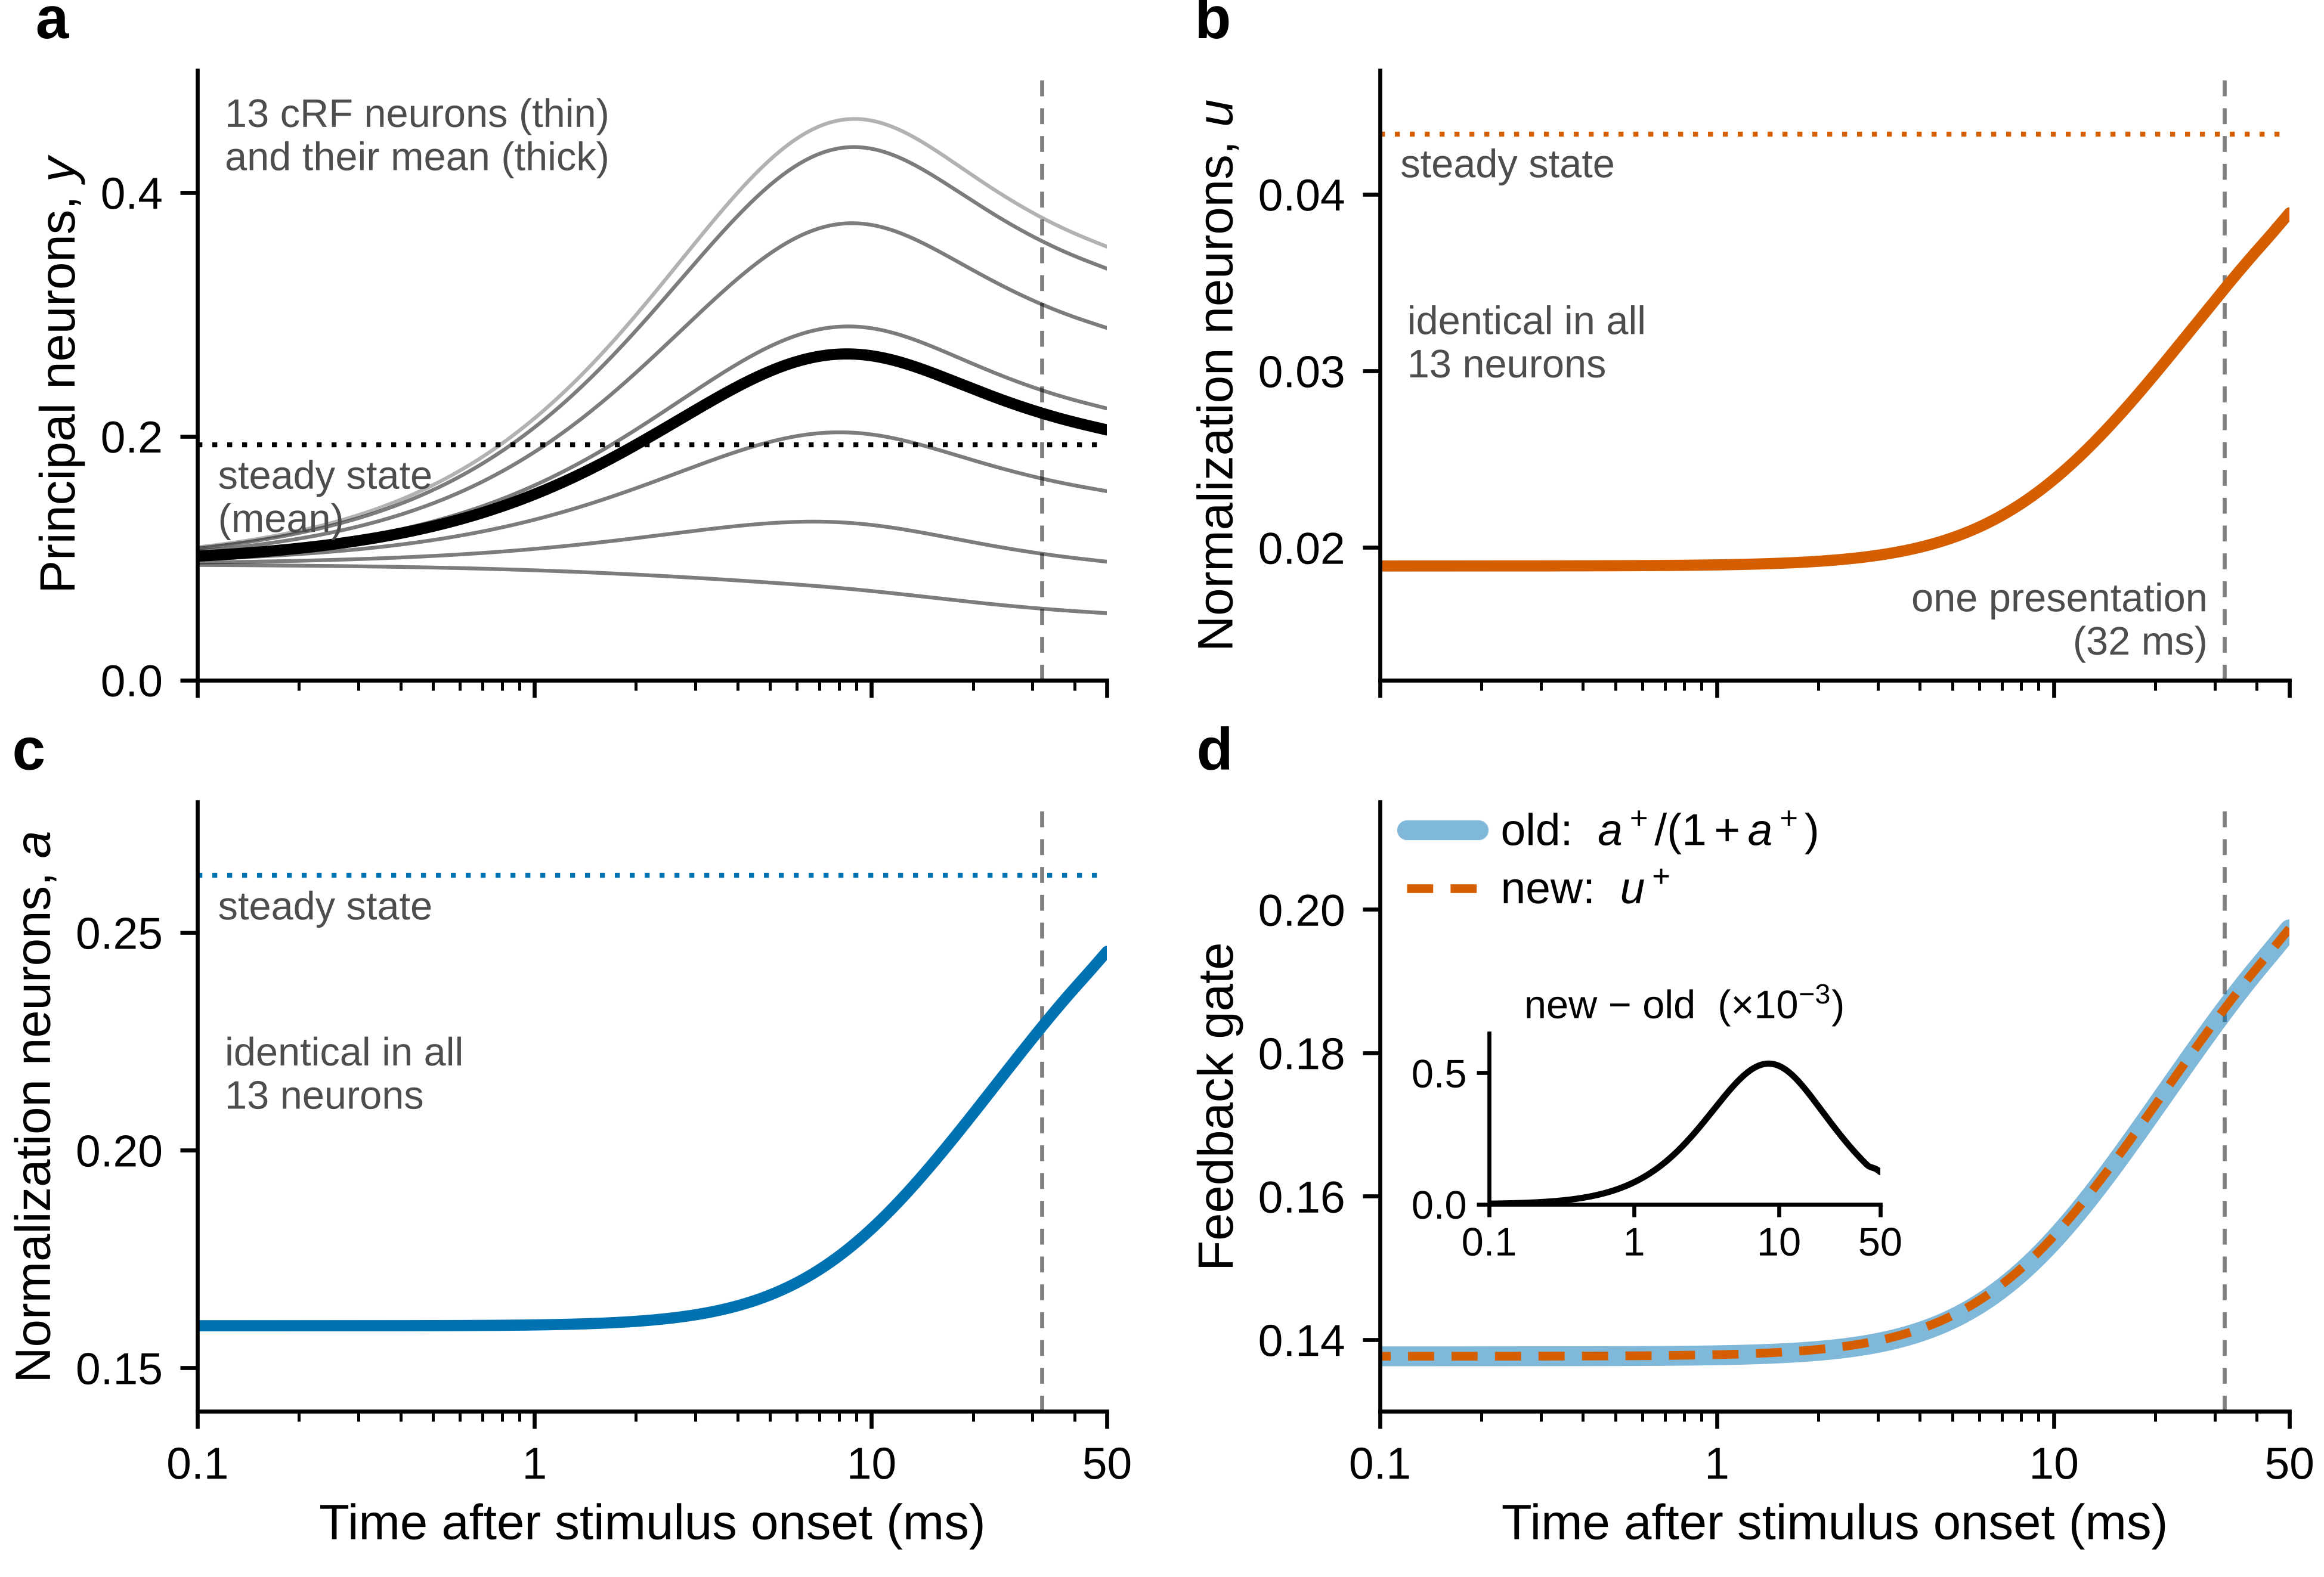
\includegraphics[width=165mm]{FigS1_timescales.png}
\caption{\textbf{Time scales of the circuit.} Responses of the 13 cRF neurons to a small grating switched on at time zero, with adaptation turned off (zero gains). \textbf{a--c}, Principal neurons $\bm{y}$ and normalization interneurons $\bm{u}$ and $\bm{a}$ against time on a logarithmic axis. Thin lines, individual neurons; thick lines, their mean; dotted lines, steady state; dashed vertical line, end of one 32~ms presentation. \textbf{d}, The two gating signals averaged across neurons; inset, their difference.}
\label{fig:timescales}
\end{figure}

\blurb{Supplementary Fig.~\ref{fig:timescales}.} We switched on a single small grating and followed each population for 50~ms. The figure shows how long each population takes to settle. The principal neurons rose within about 2~ms and then overshot, peaking at 8~ms, because the normalization signal $\bm{u}$ builds up with its 30~ms time constant. At the end of a 32~ms presentation $\bm{u}$ had completed 64\% of its change and the mean response was still 13\% above its steady state. The interneurons $\bm{a}$ followed $\bm{u}$ with no visible lag, so the old and new gates never differed by more than 0.3\%. Responses read at the end of a presentation are therefore not steady-state responses, and the two gates are interchangeable.

\begin{figure}[H]
\centering
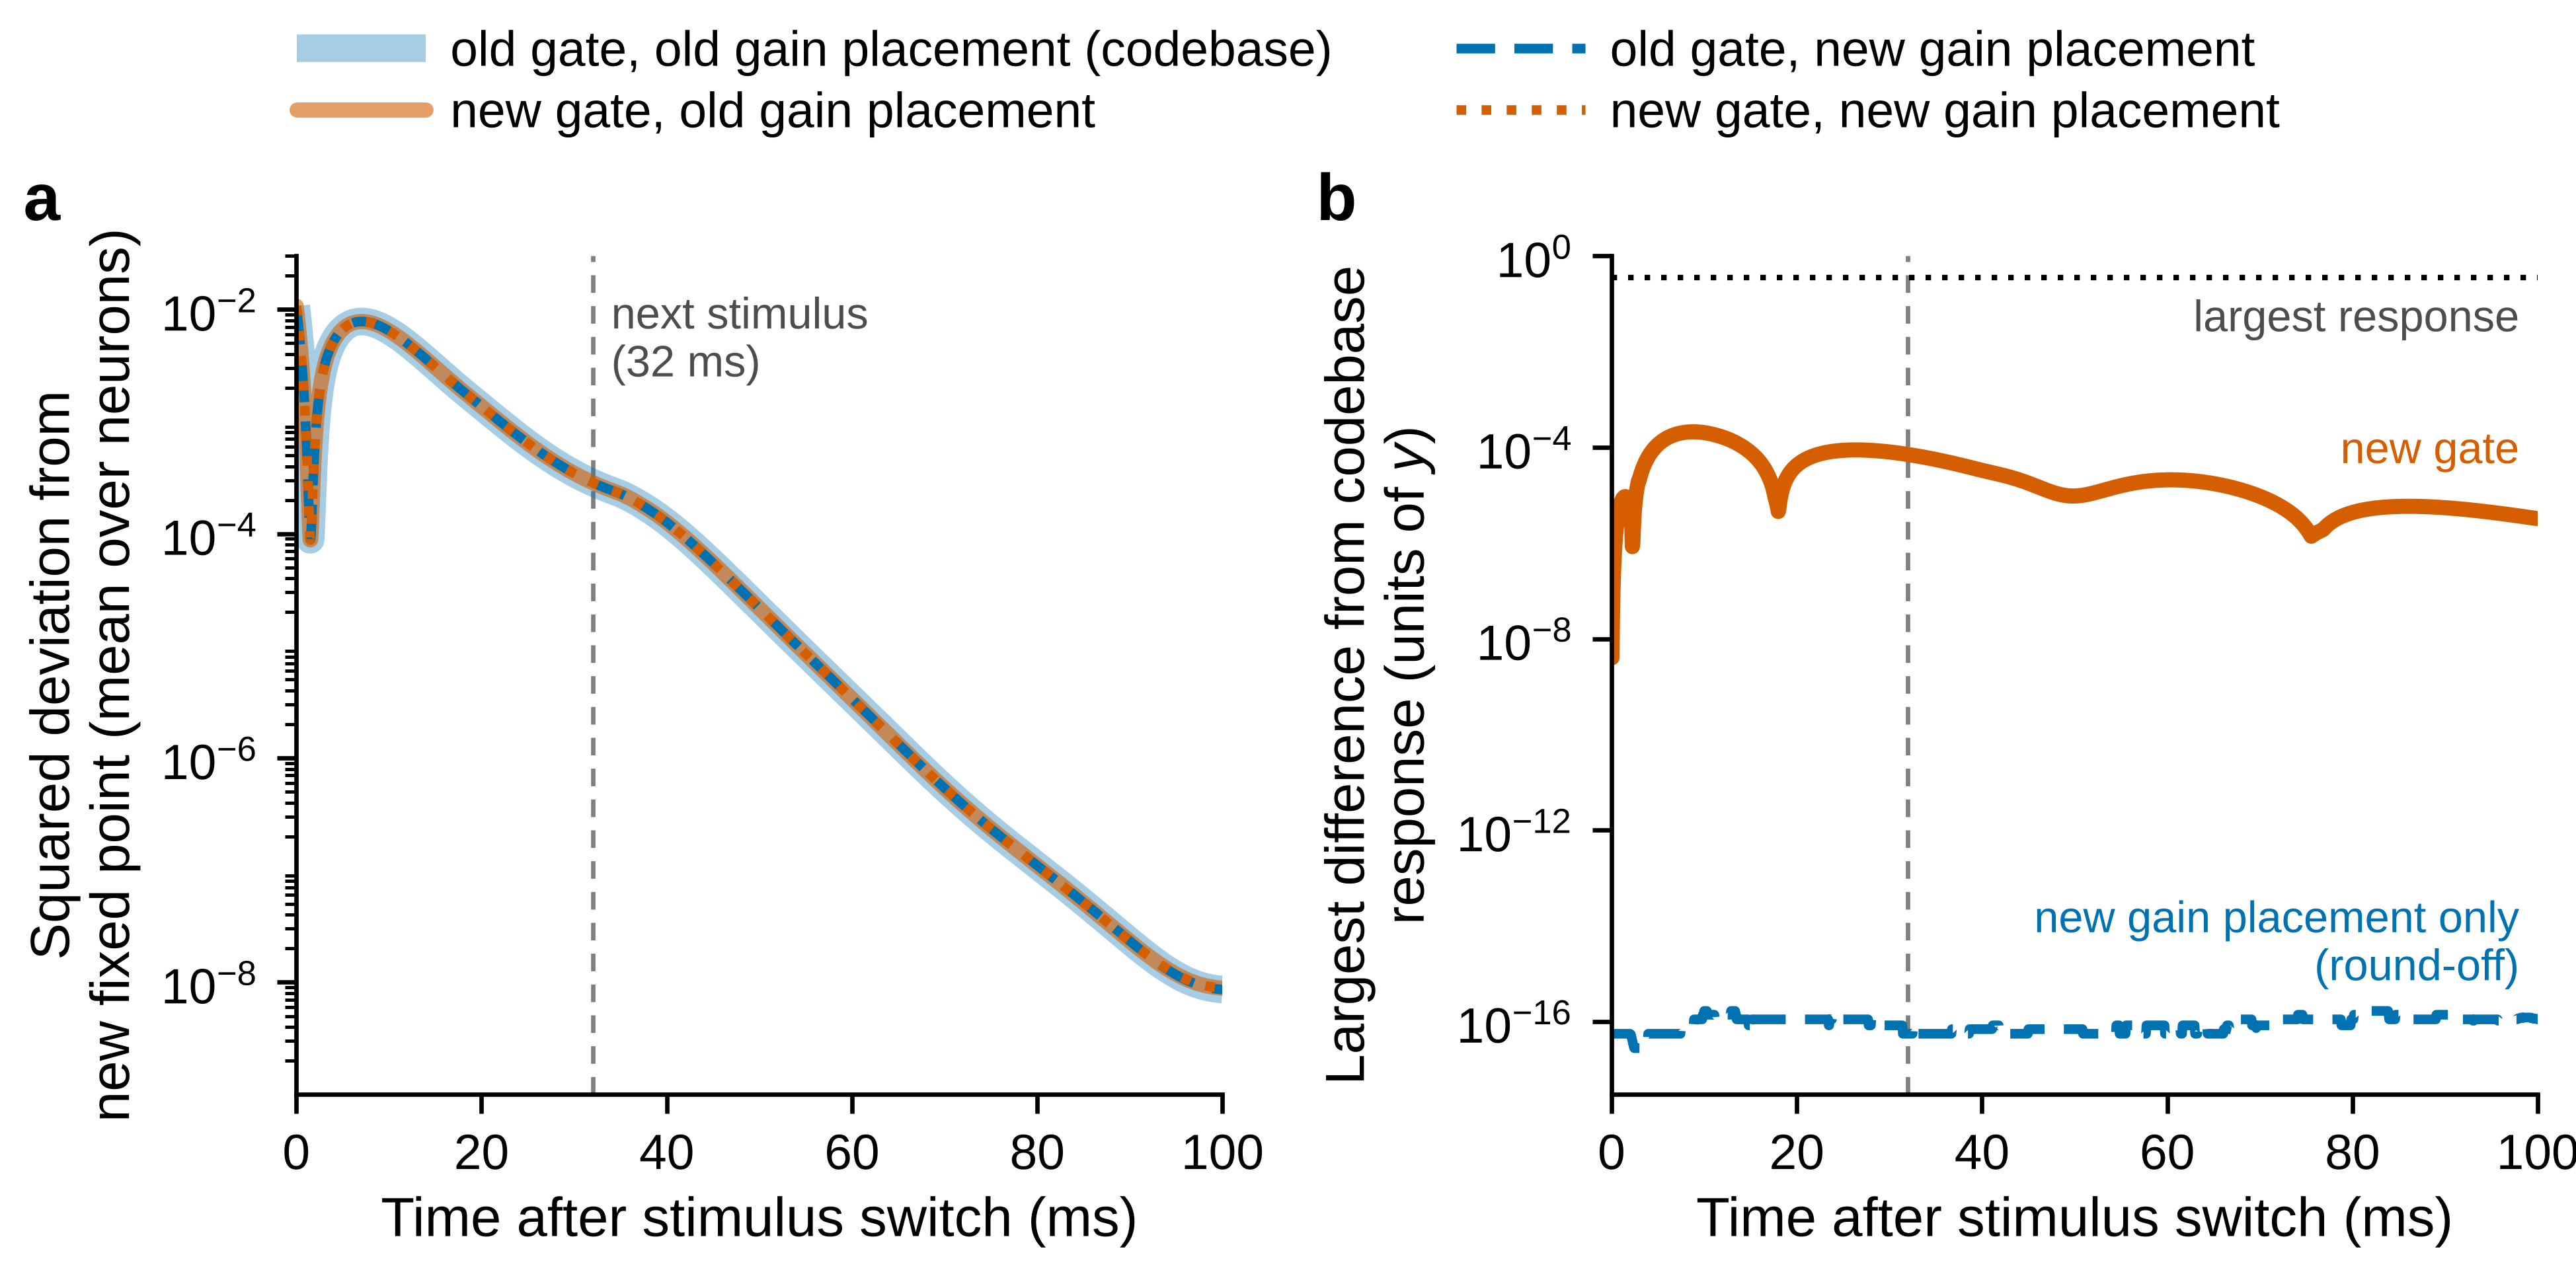
\includegraphics[width=165mm]{FigS2_settling.png}
\caption{\textbf{Settling after a change of stimulus.} Gains were frozen after adaptation to the biased ensemble. The circuit started at its steady state for one orientation and the grating switched to an orientation $55^\circ$ away at time zero. \textbf{a}, Squared distance of the cRF responses from the new steady state (mean over neurons, logarithmic axis) for the four combinations of old and new gate and gain placement. \textbf{b}, Largest difference between each variant and the earlier code. Dashed vertical lines, arrival of the next stimulus at 32~ms.}
\label{fig:settling}
\end{figure}

\blurb{Supplementary Fig.~\ref{fig:settling}.} We asked whether the gate or the placement of the gain changes how fast the circuit settles between presentations. The four curves coincide. Moving the gain into Eq.~\ref{eq:dv} is exact for frozen gains (differences at the level of round-off) and the new gate changed responses by at most $2\times10^{-4}$. In all cases the squared distance from the new steady state was still 2.7\% of its initial value when the next stimulus arrived.

\begin{figure}[H]
\centering
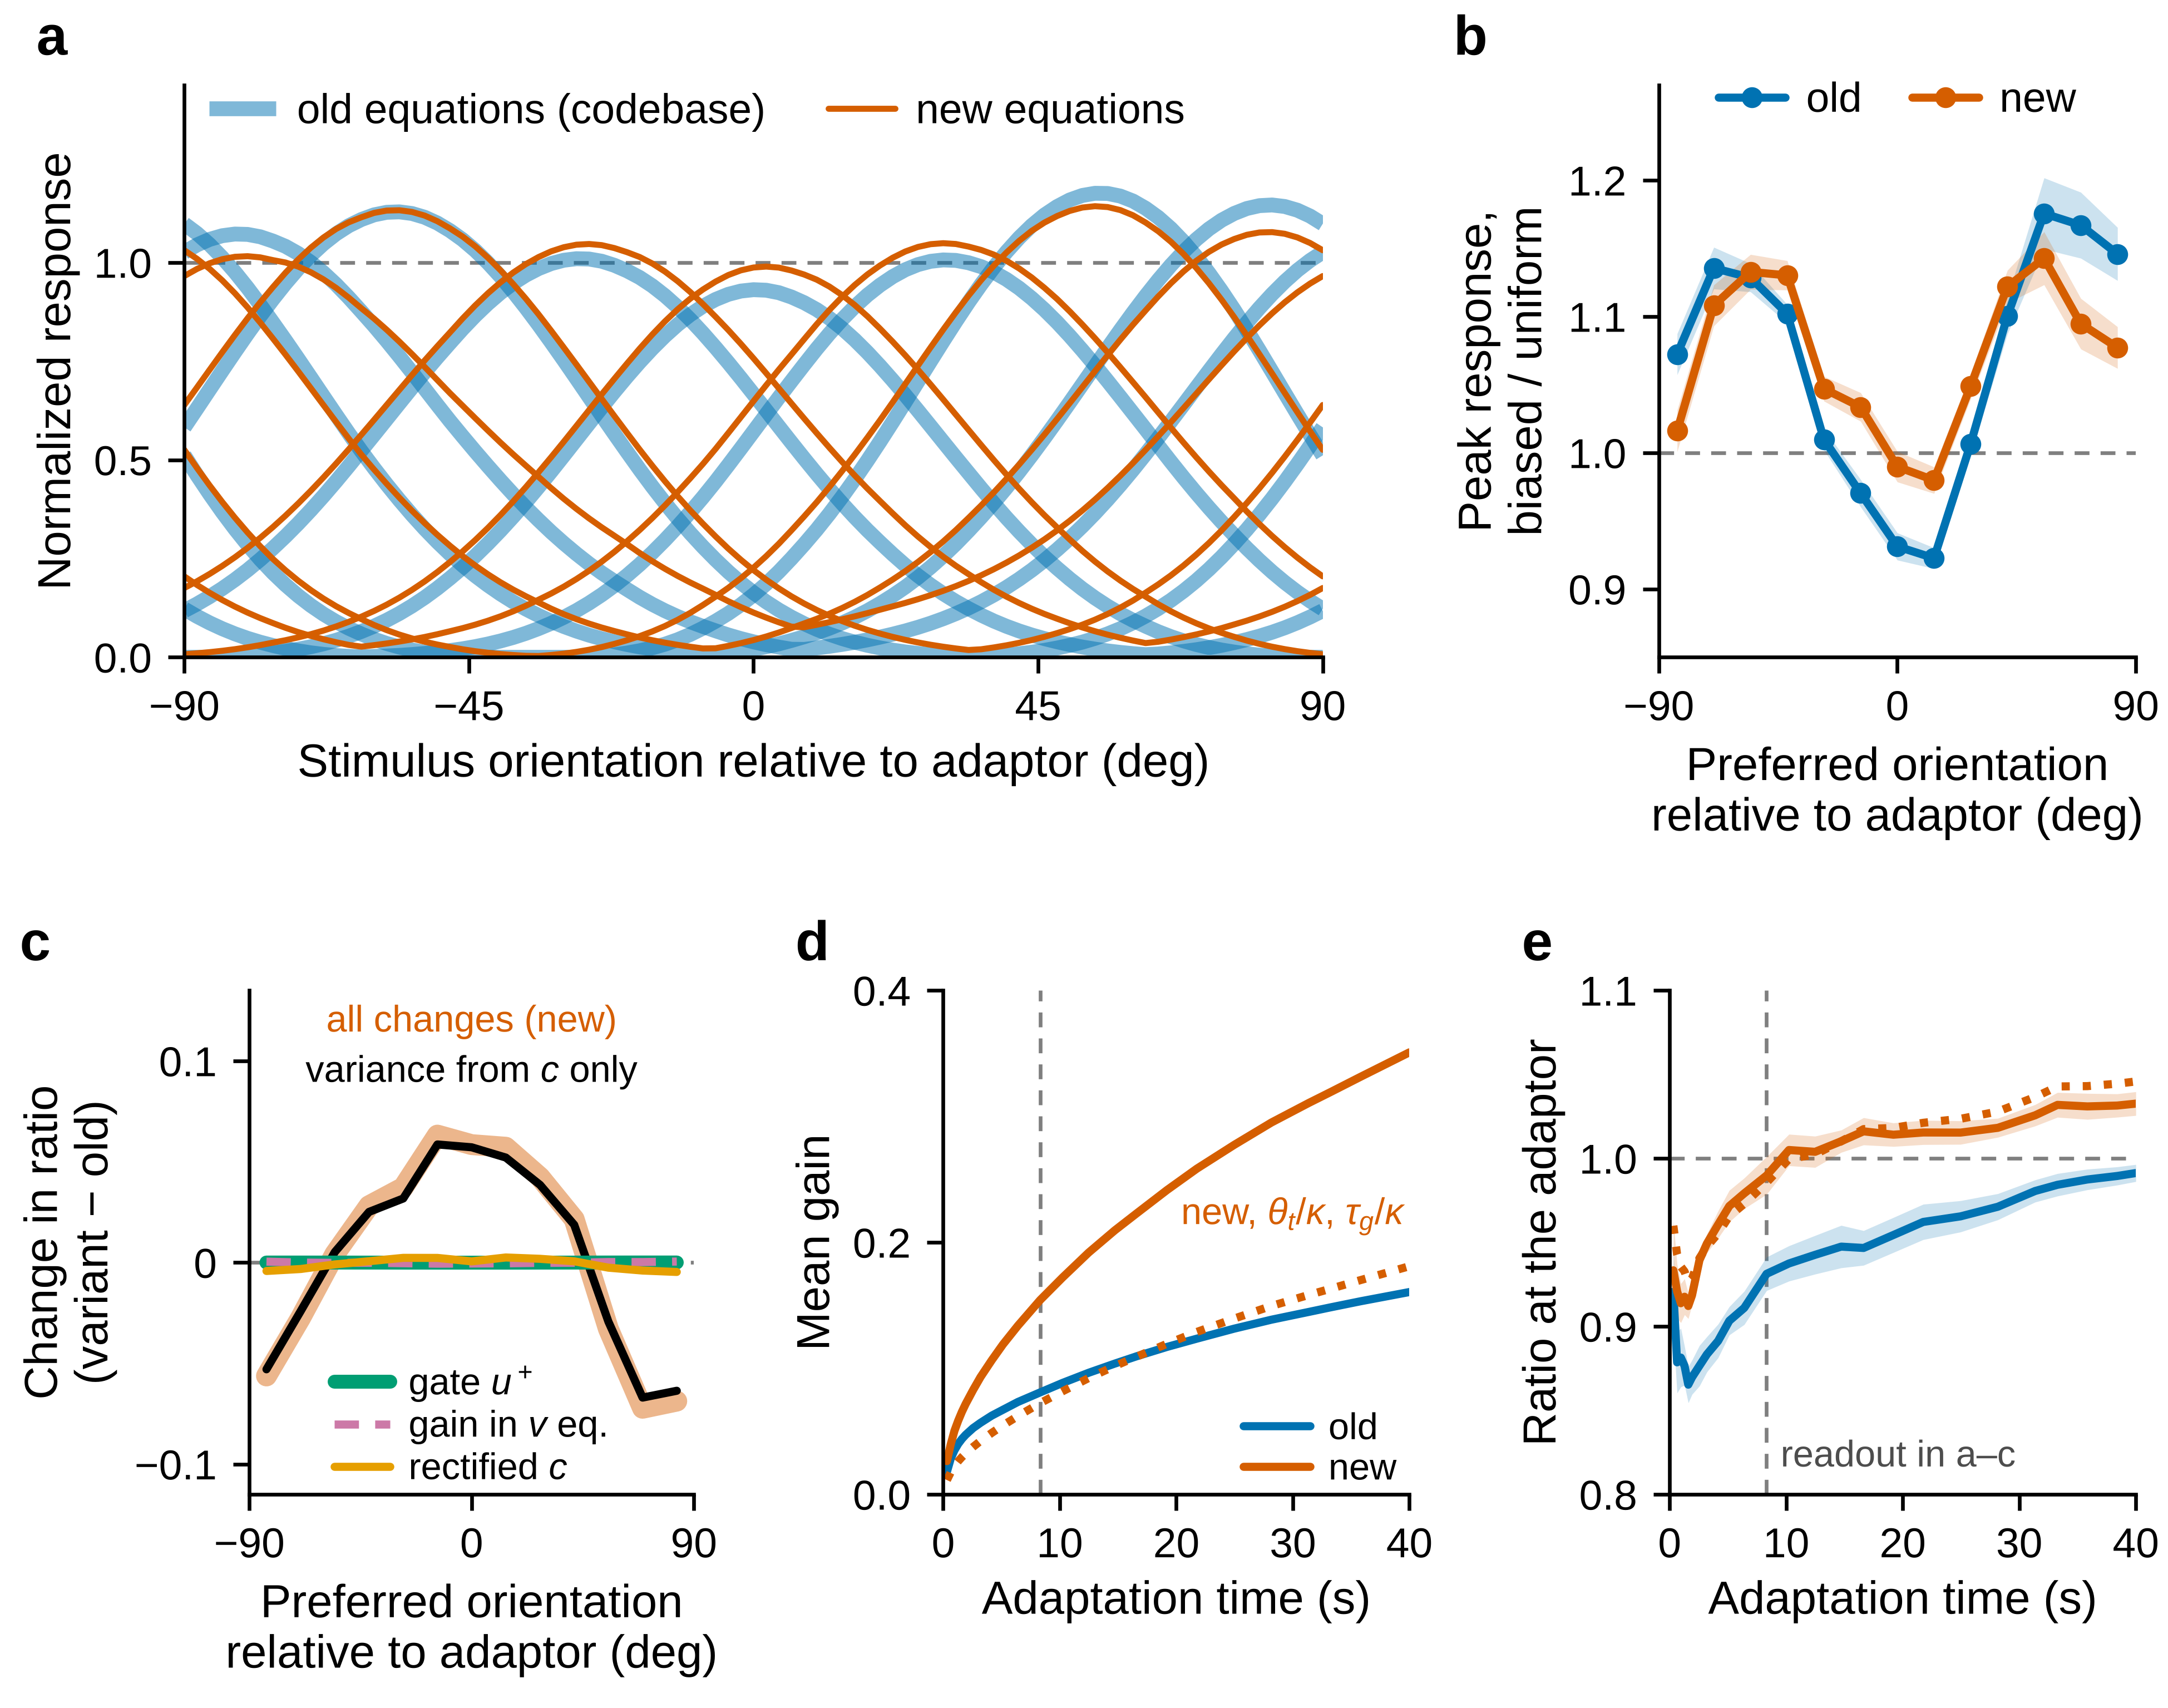
\includegraphics[width=165mm]{FigS3_tuning_old_vs_new.png}
\caption{\textbf{Tuning curves after adaptation to the biased ensemble, earlier code versus Eqs.~\ref{eq:dy}--\ref{eq:dmu}.} Small adaptors, frozen-gain readout after 8.3~s, 8 random sequences per ensemble. \textbf{a}, Tuning curves of every second cRF neuron, divided by the neuron's peak after uniform adaptation. \textbf{b}, Suppression profile (mean $\pm$ s.e.m.). \textbf{c}, Change of the profile in b caused by each change on its own. \textbf{d}, Mean gain against adaptation time; dotted, new equations with $\bm{\theta}_t$ and $\tau_g$ divided by $\kappa=0.385$, the fraction of the variance of $\bm{c}$ that passes the $\tau_v$ filter. \textbf{e}, Ratio at the adaptor against adaptation time. Dashed vertical lines in d and e, the readout time of a--c.}
\label{fig:oldnew}
\end{figure}

\blurb{Supplementary Fig.~\ref{fig:oldnew}.} We recreated Fig.~3c of the main text with the earlier code and with Eqs.~\ref{eq:dy}--\ref{eq:dmu}. The gate and the gain placement left the profile unchanged (largest change 0.0005). Driving the gains with the variance of $\bm{c}$ instead of its filtered copy roughly doubled the gains and removed most of the suppression at the adaptor (ratio $0.93\pm0.01$ with the earlier code, $0.99\pm0.01$ with the new equations). Rescaling $\bm{\theta}_t$ and $\tau_g$ by $\kappa$ restored the gains but not the suppression. Two further observations hold for both versions. The gains did not converge: they were still growing by about 1\% per second after 40~s, and by 0.3\% per second after 160~s with the new equations. And the suppression at the adaptor faded with adaptation time (panel e). Most of it arose in the first seconds, while the running mean $\bm{\mu}$ was still close to its initial value of zero and Eq.~\ref{eq:dg} was driven by the squared mean response rather than by the variance: shortening $\tau_\mu$ from 2~s to 0.2~s removed it (ratio at the adaptor 1.00 instead of 0.92 with the earlier code).

%=====================================================================
\clearpage
\suppnote{The power law and normalization}

The main text proposes that the power law of Eq.~1 of the main text breaks down at extreme probability ratios because normalization bounds response magnitude. We tested this with the protocol of Fig.~4 of the main text~\cite{tring_power_2023} (three von Mises environments, small adaptors, 30~ms presentations, 4.2~s of adaptation, large test gratings at the 13 preferred orientations, response magnitude equal to the norm of the firing rates) and Eqs.~\ref{eq:dy}--\ref{eq:dmu}.

To remove normalization we reduced the circuit to the adaptation framework of Duong et al.~\cite{duong_adaptive_2023-1}, with $\beta=1$ and the same $\bm{\theta}_t$:
\begin{align}
\tau_y \frac{d\bm{y}}{dt} &= -\bm{y} + \bm{z} - \bm{W}_{yv}\bm{v} \\
\tau_v \frac{d\bm{v}}{dt} &= -\bm{v} + \bm{g}\odot\bm{c}, \qquad \bm{c} = \bm{W}_{yv}^\top\sqrt{\bm{y}^+}
\end{align}
with Eqs.~\ref{eq:dg} and \ref{eq:dmu} unchanged. With frozen gains its steady state is $\bm{y}=[\bm{I}+\bm{W}_{yv}\bm{D}(\bm{g})\bm{W}_{yv}^\top]^{-1}\bm{z}$.

\begin{figure}[H]
\centering
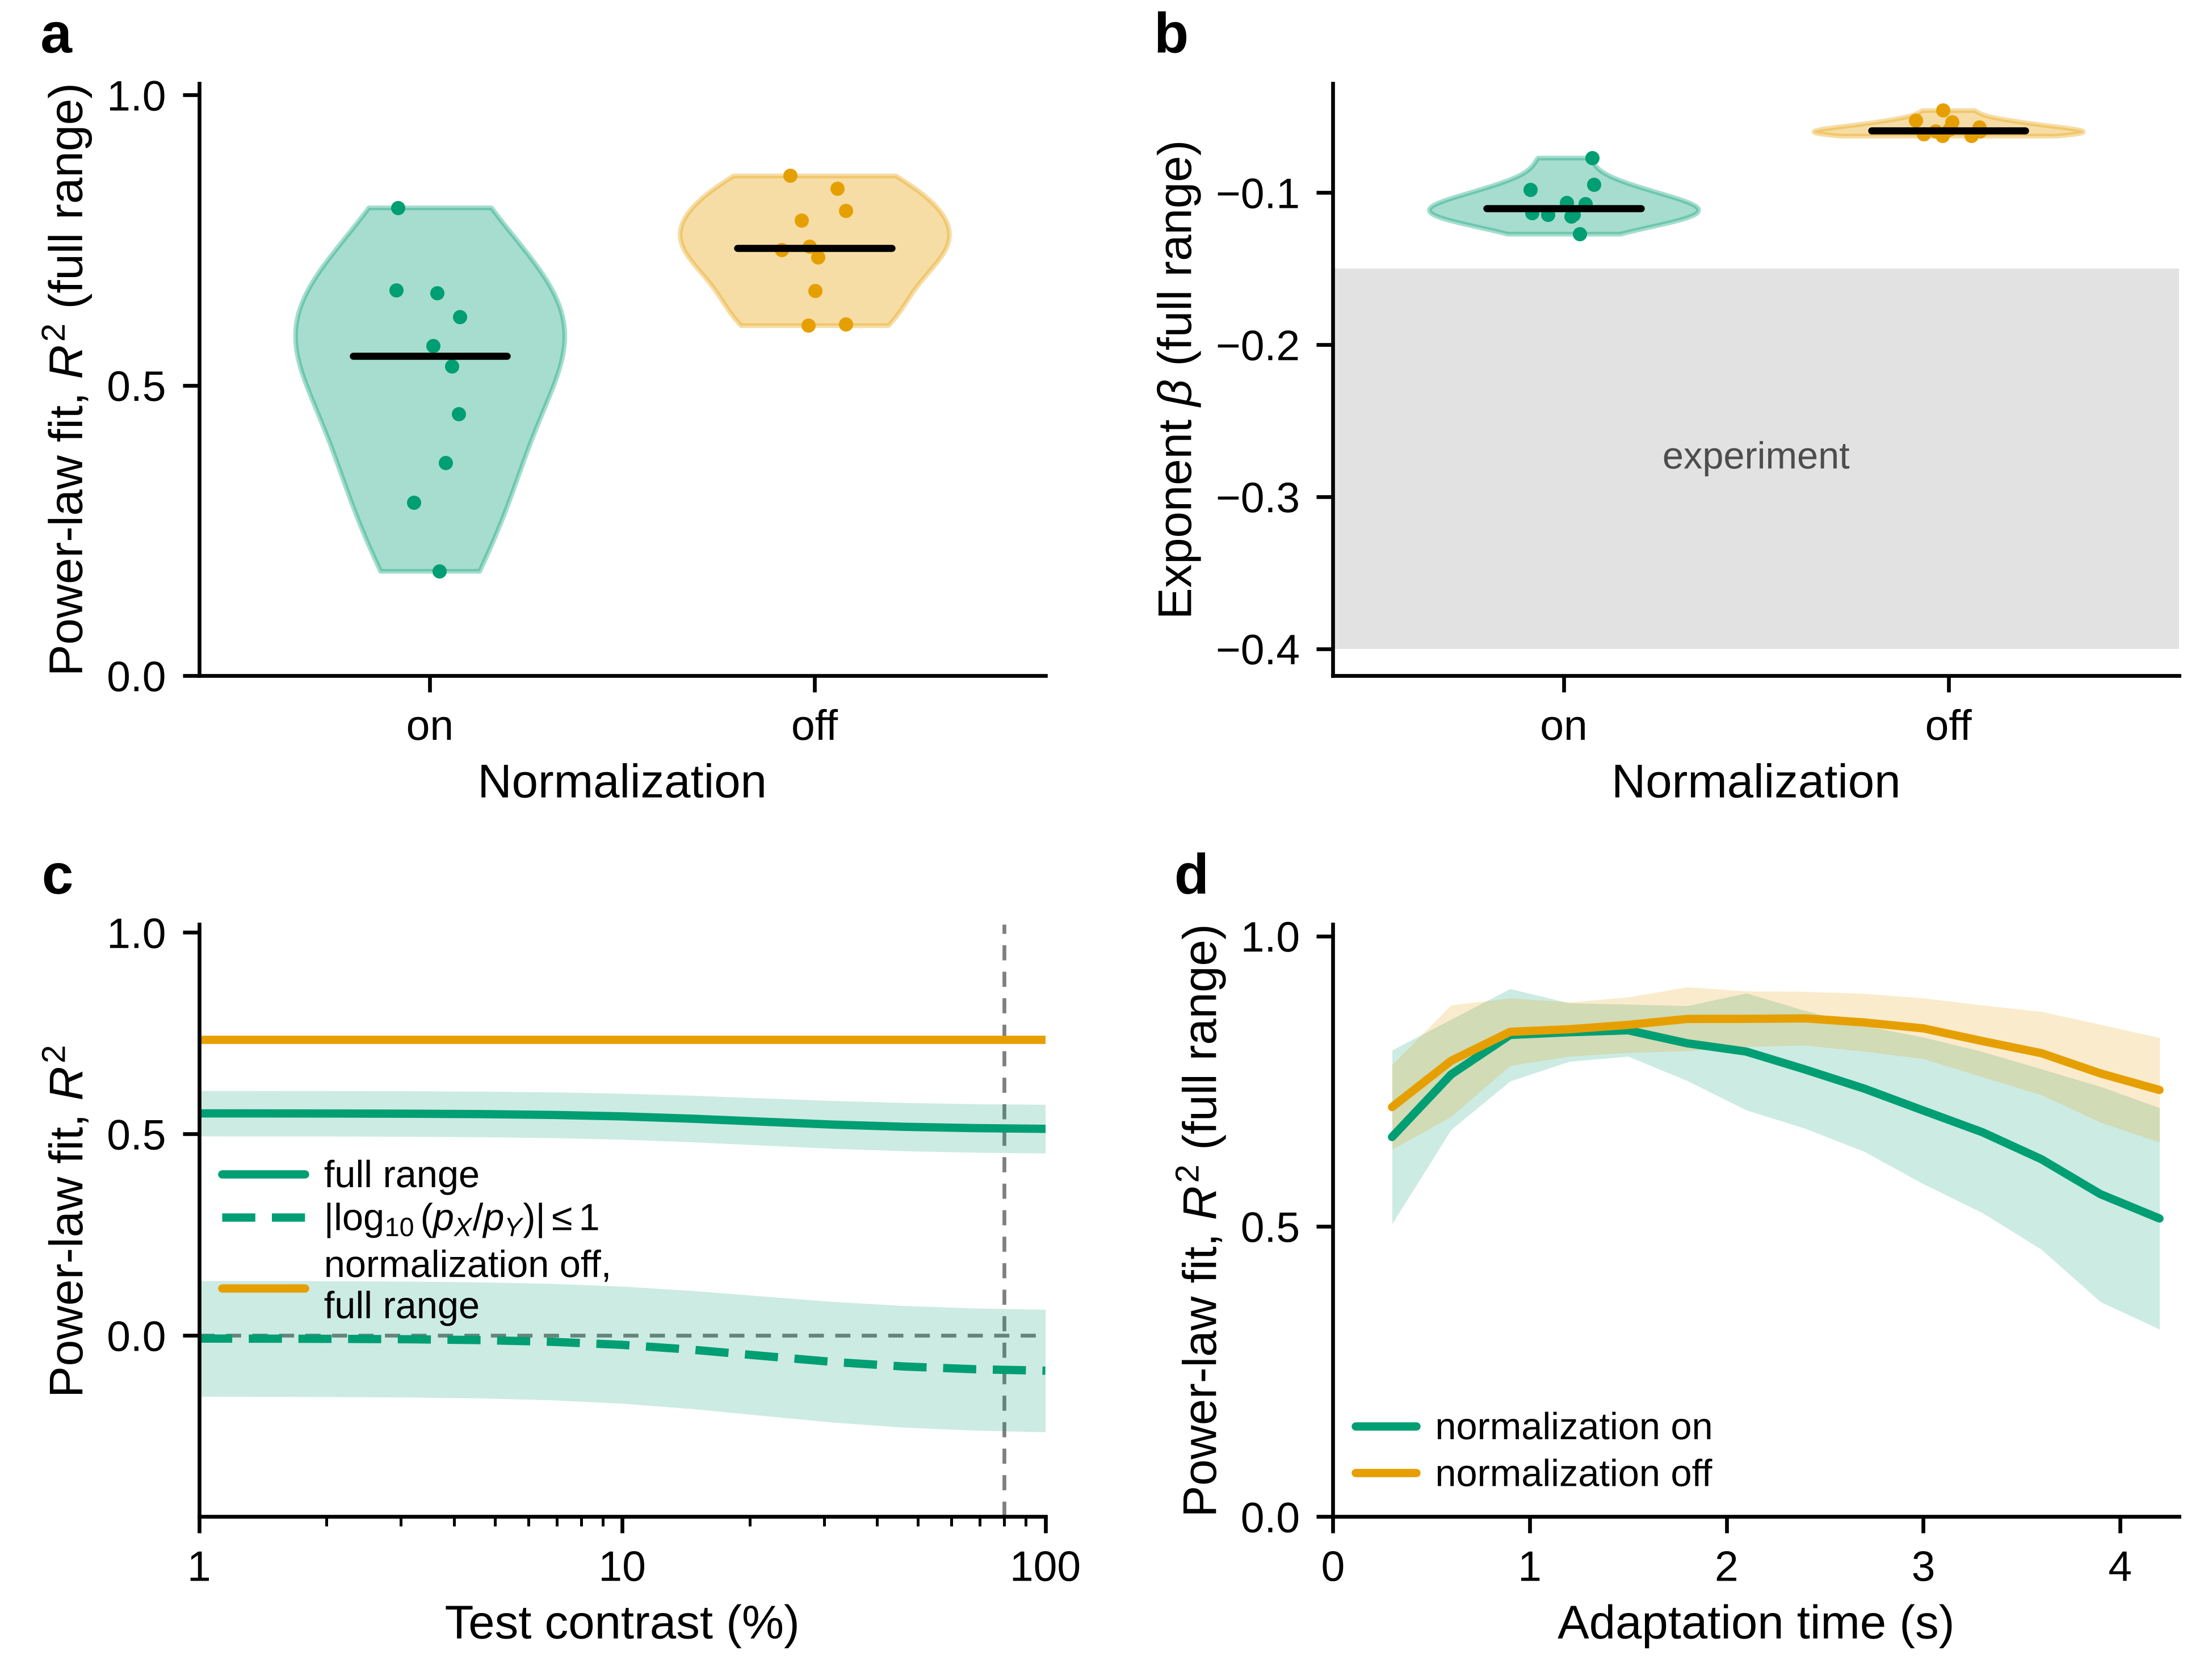
\includegraphics[width=165mm]{FigS4_power_law.png}
\caption{\textbf{Power-law fits with and without normalization.} Ten trials with different random stimulus sequences. \textbf{a}, $R^2$ of the power-law fit over the full range of probability ratios ($\log_{10}[p_X/p_Y]$ from $-1.9$ to $1.0$). Dots, trials; bars, medians. \textbf{b}, Fitted exponent $\beta$; grey band, the range reported in experiment. \textbf{c}, $R^2$ against the contrast of the test gratings (adapting contrast fixed at 80\%, dashed line), for the full range and for $|\log_{10}[p_X/p_Y]|\le1$; mean $\pm$ s.e.m. \textbf{d}, $R^2$ (full range) against adaptation time; mean $\pm$ s.d.}
\label{fig:powerlaw}
\end{figure}

\blurb{Supplementary Fig.~\ref{fig:powerlaw}.} We adapted the circuit to the three environments with normalization on and off and fitted the power law to the response ratios. The figure shows whether removing normalization, or weakening it with low test contrast, restores the power law. It did not. After 4.2~s the fit over the full range was poor in both cases ($R^2=0.51\pm0.19$ with normalization, $0.74\pm0.09$ without; mean $\pm$ s.d.), and within $|\log_{10}[p_X/p_Y]|\le1$ it was worse ($R^2=-0.08$ and $0.53$). The exponents ($\beta=-0.11\pm0.01$ and $-0.06\pm0.01$) fell outside the experimental range of $[-0.4,-0.15]$. Lowering the test contrast to 1\% changed $R^2$ by 0.04. In both cases the fit was best after about 1.5~s ($R^2\approx0.84$) and degraded as adaptation continued. Normalization therefore lowers the quality of the fit but does not cause the breakdown. The gains were still growing at the end of adaptation (by 12\% and 8\% per second), so these values describe a transient state. With the equations of the earlier code the same protocol gave $\beta=-0.15\pm0.02$ and $R^2=0.91\pm0.04$ within $|\log_{10}[p_X/p_Y]|\le1$, and $\beta=-0.12\pm0.01$ and $R^2=0.91\pm0.03$ over the full range.

\subsection*{Does a covariance transformation alone produce a power law?}

We next asked a simpler question that involves no circuit: if responses are produced by the exact transformation that maps the input covariance onto the target covariance, is $\log(r_X/r_Y)$ a linear function of $\log(p_X/p_Y)$? For each environment $X$ we computed the covariance $\bm{\Sigma}_X$ of the input drive and the unique symmetric positive-definite matrix that satisfies $\bm{M}_X\bm{\Sigma}_X\bm{M}_X=\bm{\Sigma}_t$,
\begin{equation}
\bm{M}_X = \bm{\Sigma}_X^{-1/2}\left(\bm{\Sigma}_X^{1/2}\,\bm{\Sigma}_t\,\bm{\Sigma}_X^{1/2}\right)^{1/2}\bm{\Sigma}_X^{-1/2},
\end{equation}
and took $\bm{M}_X\bm{z}(s)$ as the response to stimulus $s$. Scaling $\bm{\Sigma}_t$ by a constant scales every $\bm{M}_X$ equally and cancels in $r_X/r_Y$, so only the shape of the target can matter.

\begin{figure}[H]
\centering
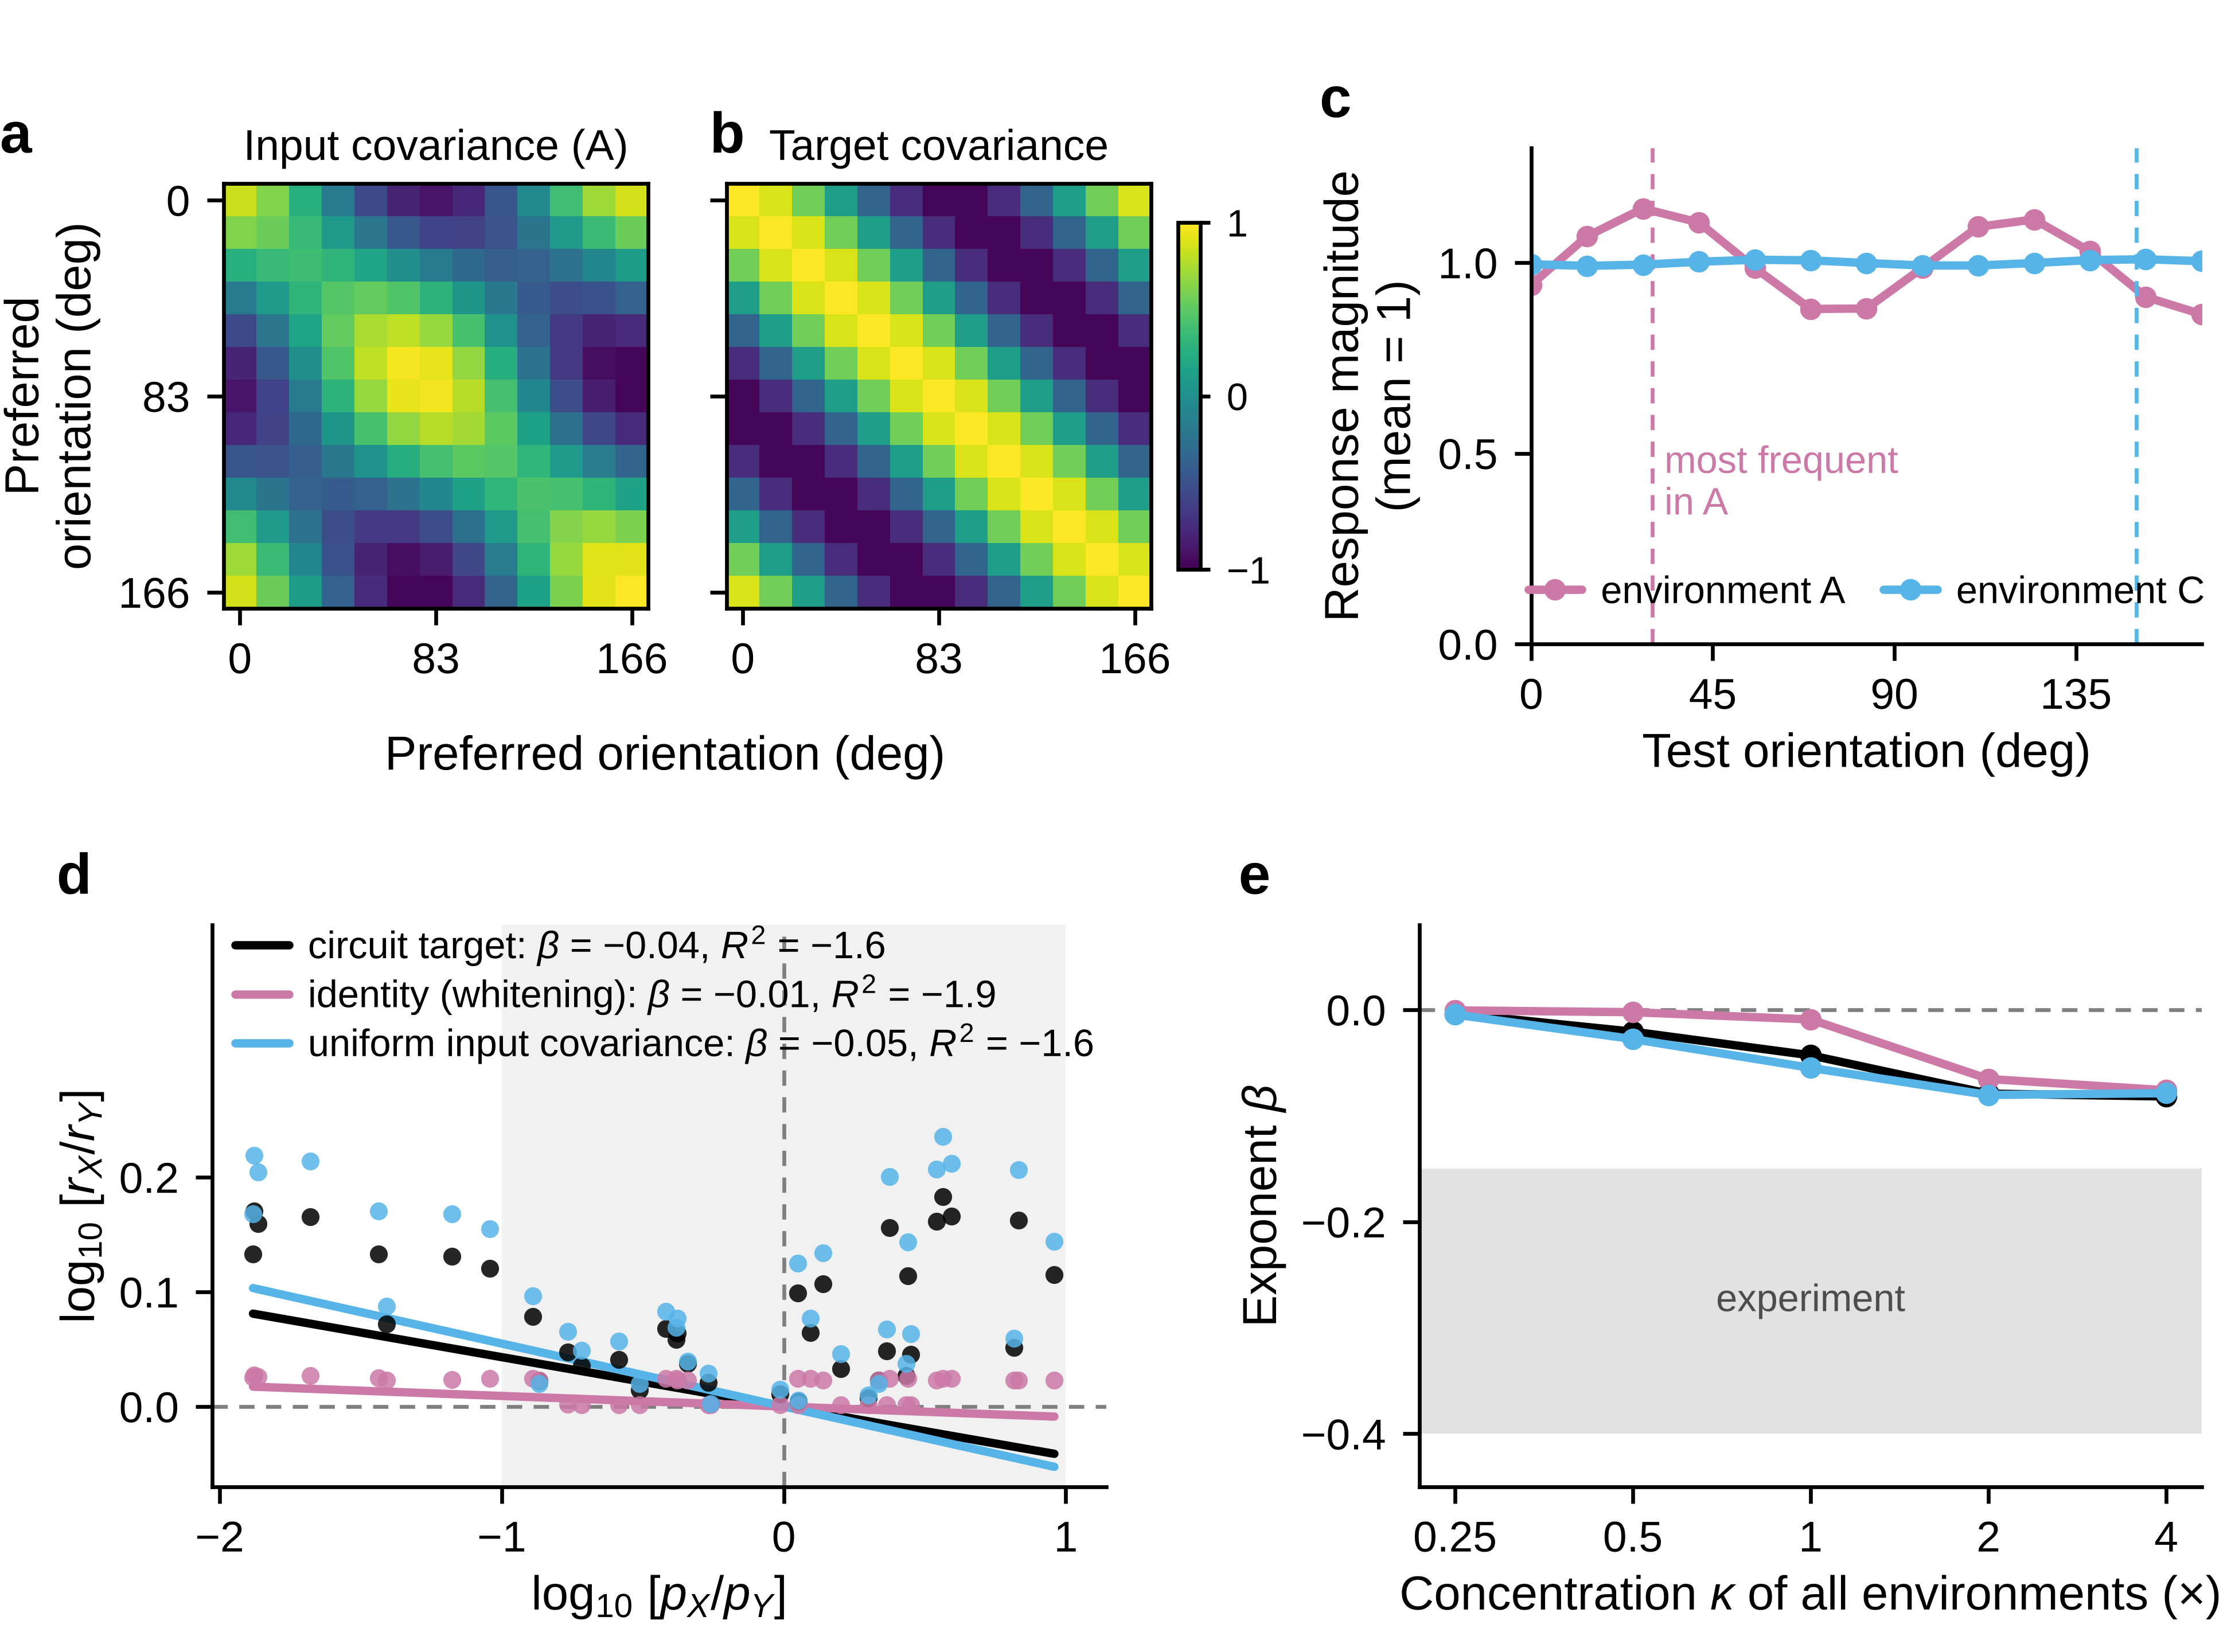
\includegraphics[width=165mm]{FigS5_covariance_transform.png}
\caption{\textbf{Responses under an exact covariance transformation.} \textbf{a}, Covariance of the input drive in environment A (most frequent orientation $30^\circ$). \textbf{b}, Target covariance of the circuit. Both are normalized to their largest entry. \textbf{c}, Response magnitude after the exact transformation against test orientation, for the most and least peaked environments; dashed lines, the most frequent orientation of each. \textbf{d}, Log response ratio against log probability ratio for three targets, with power-law fits; grey region, $|\log_{10}[p_X/p_Y]|\le1$. \textbf{e}, Fitted exponent when the concentration of all three environments is scaled; grey band, experiment.}
\label{fig:covtransform}
\end{figure}

\blurb{Supplementary Fig.~\ref{fig:covtransform}.} We applied the exact transformation to the inputs and repeated the power-law analysis. The figure shows whether matching covariance is enough to produce the power law. It is not. The response ratio did not follow the probability ratio: the points formed a V rather than a line (panel d), the fitted exponent stayed between $-0.09$ and $0$ for every target and every concentration (panel e), and $R^2$ was negative, meaning that the power law fitted worse than a constant. Responses were largest both at the most frequent orientation and at the orientation orthogonal to it (panel c). The result did not depend on the target (circuit target, identity, or the covariance of uniformly distributed inputs). The input covariance was nearly rank two, so we added a ridge of $10^{-6}$ times its mean eigenvalue; ridges from $10^{-10}$ to $10^{-2}$ moved $\beta$ between $-0.01$ and $-0.13$, depending on the target, and never produced a positive $R^2$.

The reason is that the transformation is defined by second-order statistics but is applied to the raw inputs. Covariance measures how responses vary around their mean, and it changes in the same way for stimuli that are much more frequent and much less frequent than average. The power law instead concerns mean response magnitude, a first-order statistic. In our stimuli 79\% of the squared input drive lies along the direction in which all neurons respond equally, and this direction carries almost no variance (less than $10^{-5}$ of the total), so the covariance leaves the largest part of the response unconstrained. A covariance transformation alone therefore does not predict the power law; where the circuit follows it, it does so through the transient described in Supplementary Note~1.

%=====================================================================
\clearpage
\suppnote{The suppression profile under biased ensembles}

Benucci et al.~\cite{benucci_adaptation_2013} reported weak suppression at all orientations and strong suppression at the adaptor. With gains active during adaptation to both ensembles the circuit did not produce this pattern (Supplementary Fig.~\ref{fig:oldnew}b): responses far from the adaptor were facilitated by about 10\%.

The variance of the input explains why. Let neuron $i$ have mean drive $\bar z_i$ and variance $V_i$ under the uniform ensemble, and let the biased ensemble show the adaptor on an extra fraction $q$ of presentations. The variance of its drive under the biased ensemble is
\begin{equation}
V_i^{\text{biased}} = (1-q)\,V_i + q(1-q)\left(z_i(\theta_{\text{adaptor}})-\bar z_i\right)^2 .
\label{eq:variance}
\end{equation}
The second term is large for neurons that respond much more than average to the adaptor and equally large for neurons that respond much less than average to it. For our stimuli ($q=\tfrac13$) the variance rose by 11\% for neurons tuned to the adaptor and by the same 11\% for neurons tuned to the orthogonal orientation, fell by up to 33\% for neurons on the flanks ($\pm42^\circ$), and fell by 11\% in total. A mechanism that holds variance at a fixed target therefore suppresses the adaptor and the orthogonal orientation equally and releases the flanks. It cannot single out the adaptor at steady state. We tested three additions that might change this.

To compare profiles we used the root-mean-square distance between the simulated profile and a target profile, $0.9-0.3\exp(-\Delta\theta^2/2w^2)$ with $w=20^\circ$. We did not have access to the original data, so these values are nominal: they encode weak untuned suppression (ratio 0.9) and strong suppression at the adaptor (ratio 0.6). We also report the ratio far from the adaptor ($|\Delta\theta|\ge55^\circ$) and at the adaptor, which do not depend on these values.

\begin{figure}[H]
\centering
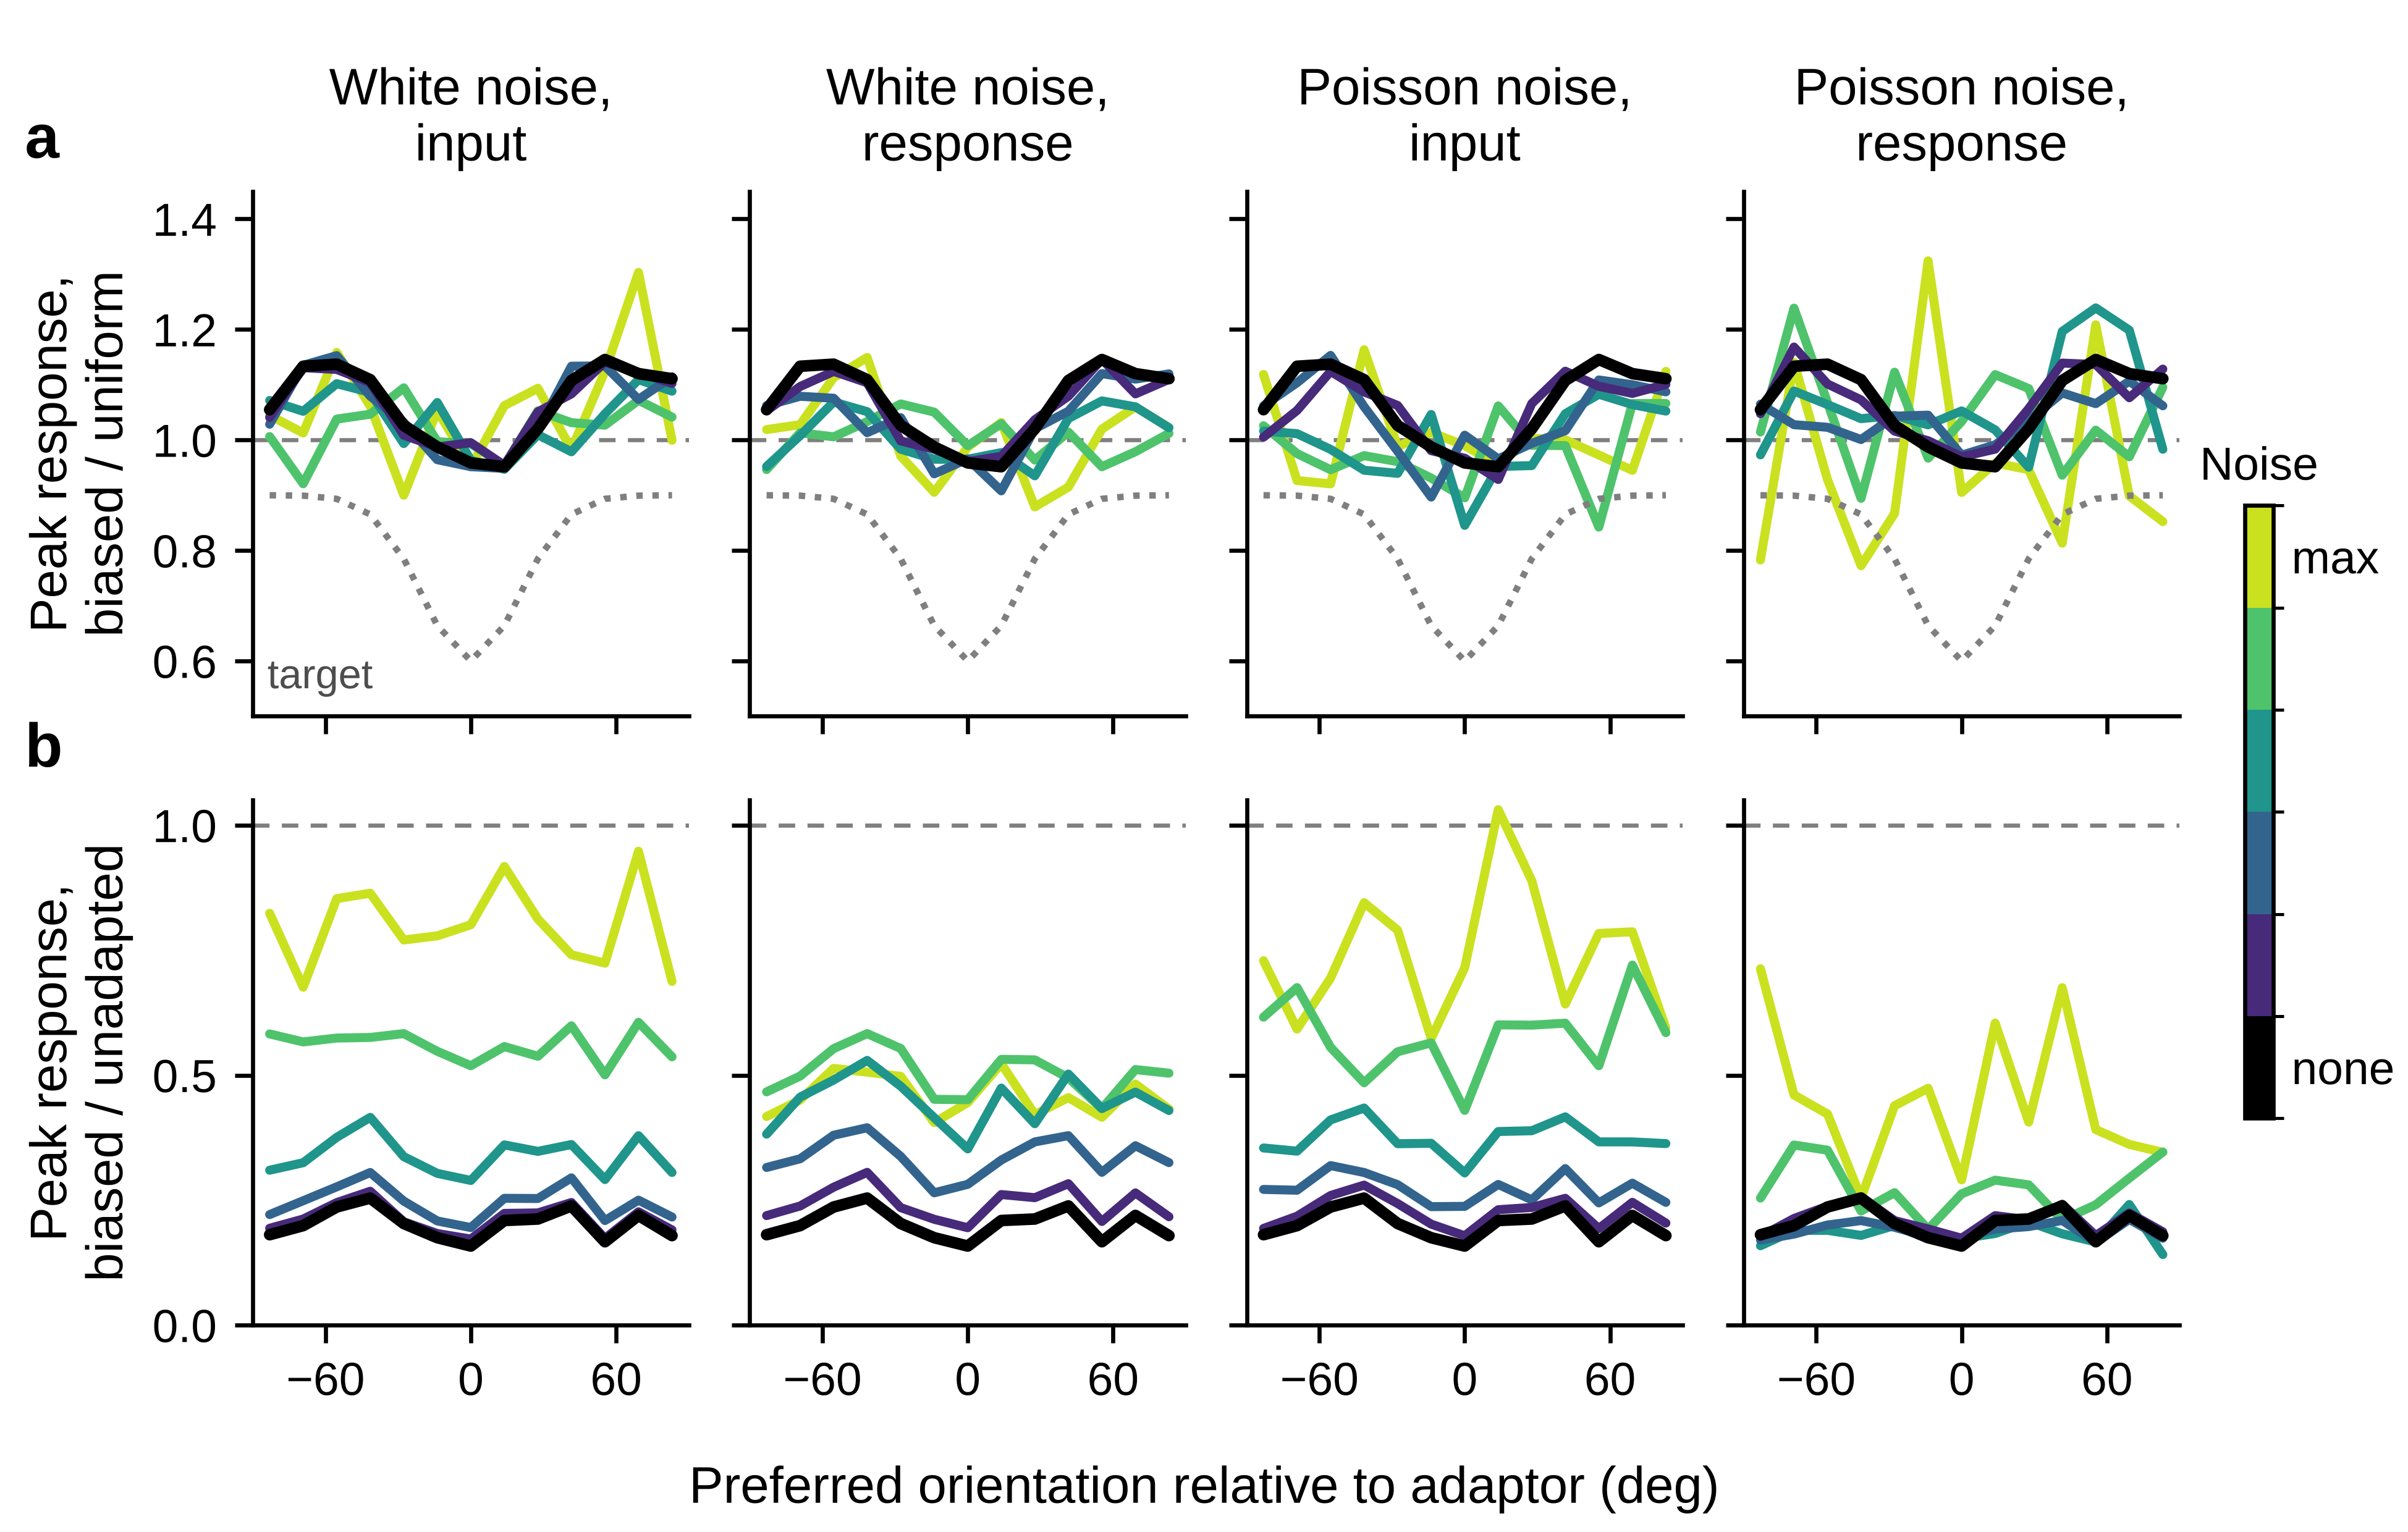
\includegraphics[width=165mm]{FigS6_noise.png}
\caption{\textbf{Effect of noise on the suppression profile.} Small adaptors, frozen-gain readout, 4 random sequences per ensemble; noise was present during adaptation and readout. Columns, type of noise. Black, no noise; colors, five increasing noise levels. White noise: standard deviation up to 0.8 (input) or 0.24 (response) times the peak unadapted input or response, after 1~ms low-pass filtering. Poisson noise: counts in 1~ms bins with rate scales down to 300 (input) or 1000 (response) spikes per second at the peak unadapted input or firing rate. \textbf{a}, Profile relative to the uniform-adapted state; dotted, target. \textbf{b}, Profile relative to the unadapted circuit at the same noise level.}
\label{fig:noise}
\end{figure}

\blurb{Supplementary Fig.~\ref{fig:noise}.} We injected noise into the dynamics, so that it reached the variance interneurons and the gains, and measured the suppression profile at six noise levels. The hypothesis was that noise adds variance to all neurons, raises all gains, and so produces untuned suppression. The figure shows the profile against preferred orientation for each noise type and level. Poisson noise did raise the gains (by up to 65\% for input noise and 79\% for response noise), but it raised them equally for the uniform and biased ensembles, so the ratio far from the adaptor stayed between 0.97 and 1.12 at every level (panel a). White input noise lowered the gains slightly (by 13\%), because it strengthened normalization, and white response noise changed them by less than 10\%. Relative to the unadapted circuit (panel b) suppression was already strong and untuned without noise (ratio 0.16--0.20), and noise mostly weakened it. Noise does not produce untuned suppression relative to the uniform-adapted state. Results did not depend on the time step: repeating the white-noise runs with half the step gave the same mean gain to within 1\%.

Next we replaced the all-ones normalization weights by Gaussian profiles in space and orientation,
\begin{equation}
N_{ij} \propto \exp\!\left(-\frac{d_{ij}^2}{2\sigma_s^2}\right)\exp\!\left(-\frac{\Delta\theta_{ij}^2}{2\sigma_\theta^2}\right),
\end{equation}
where $d_{ij}$ is the distance between RF centers in cRF diameters (surround RFs abutting the cRF) and $\Delta\theta_{ij}$ the difference in preferred orientation. $\bm{N}$ was rescaled so that the cRF neuron tuned to an adapting grating received the same pooled drive as with all-ones weights. Its unadapted response to that grating was then identical; across contrasts from 1\% to 100\% its response stayed within a factor 1.6 of the all-ones case for the narrowest pools and within 1.25 for $\sigma_s\ge2$. Because non-uniform weights break the analytic fixed point, all responses were obtained by integrating the full dynamics.

\begin{figure}[H]
\centering
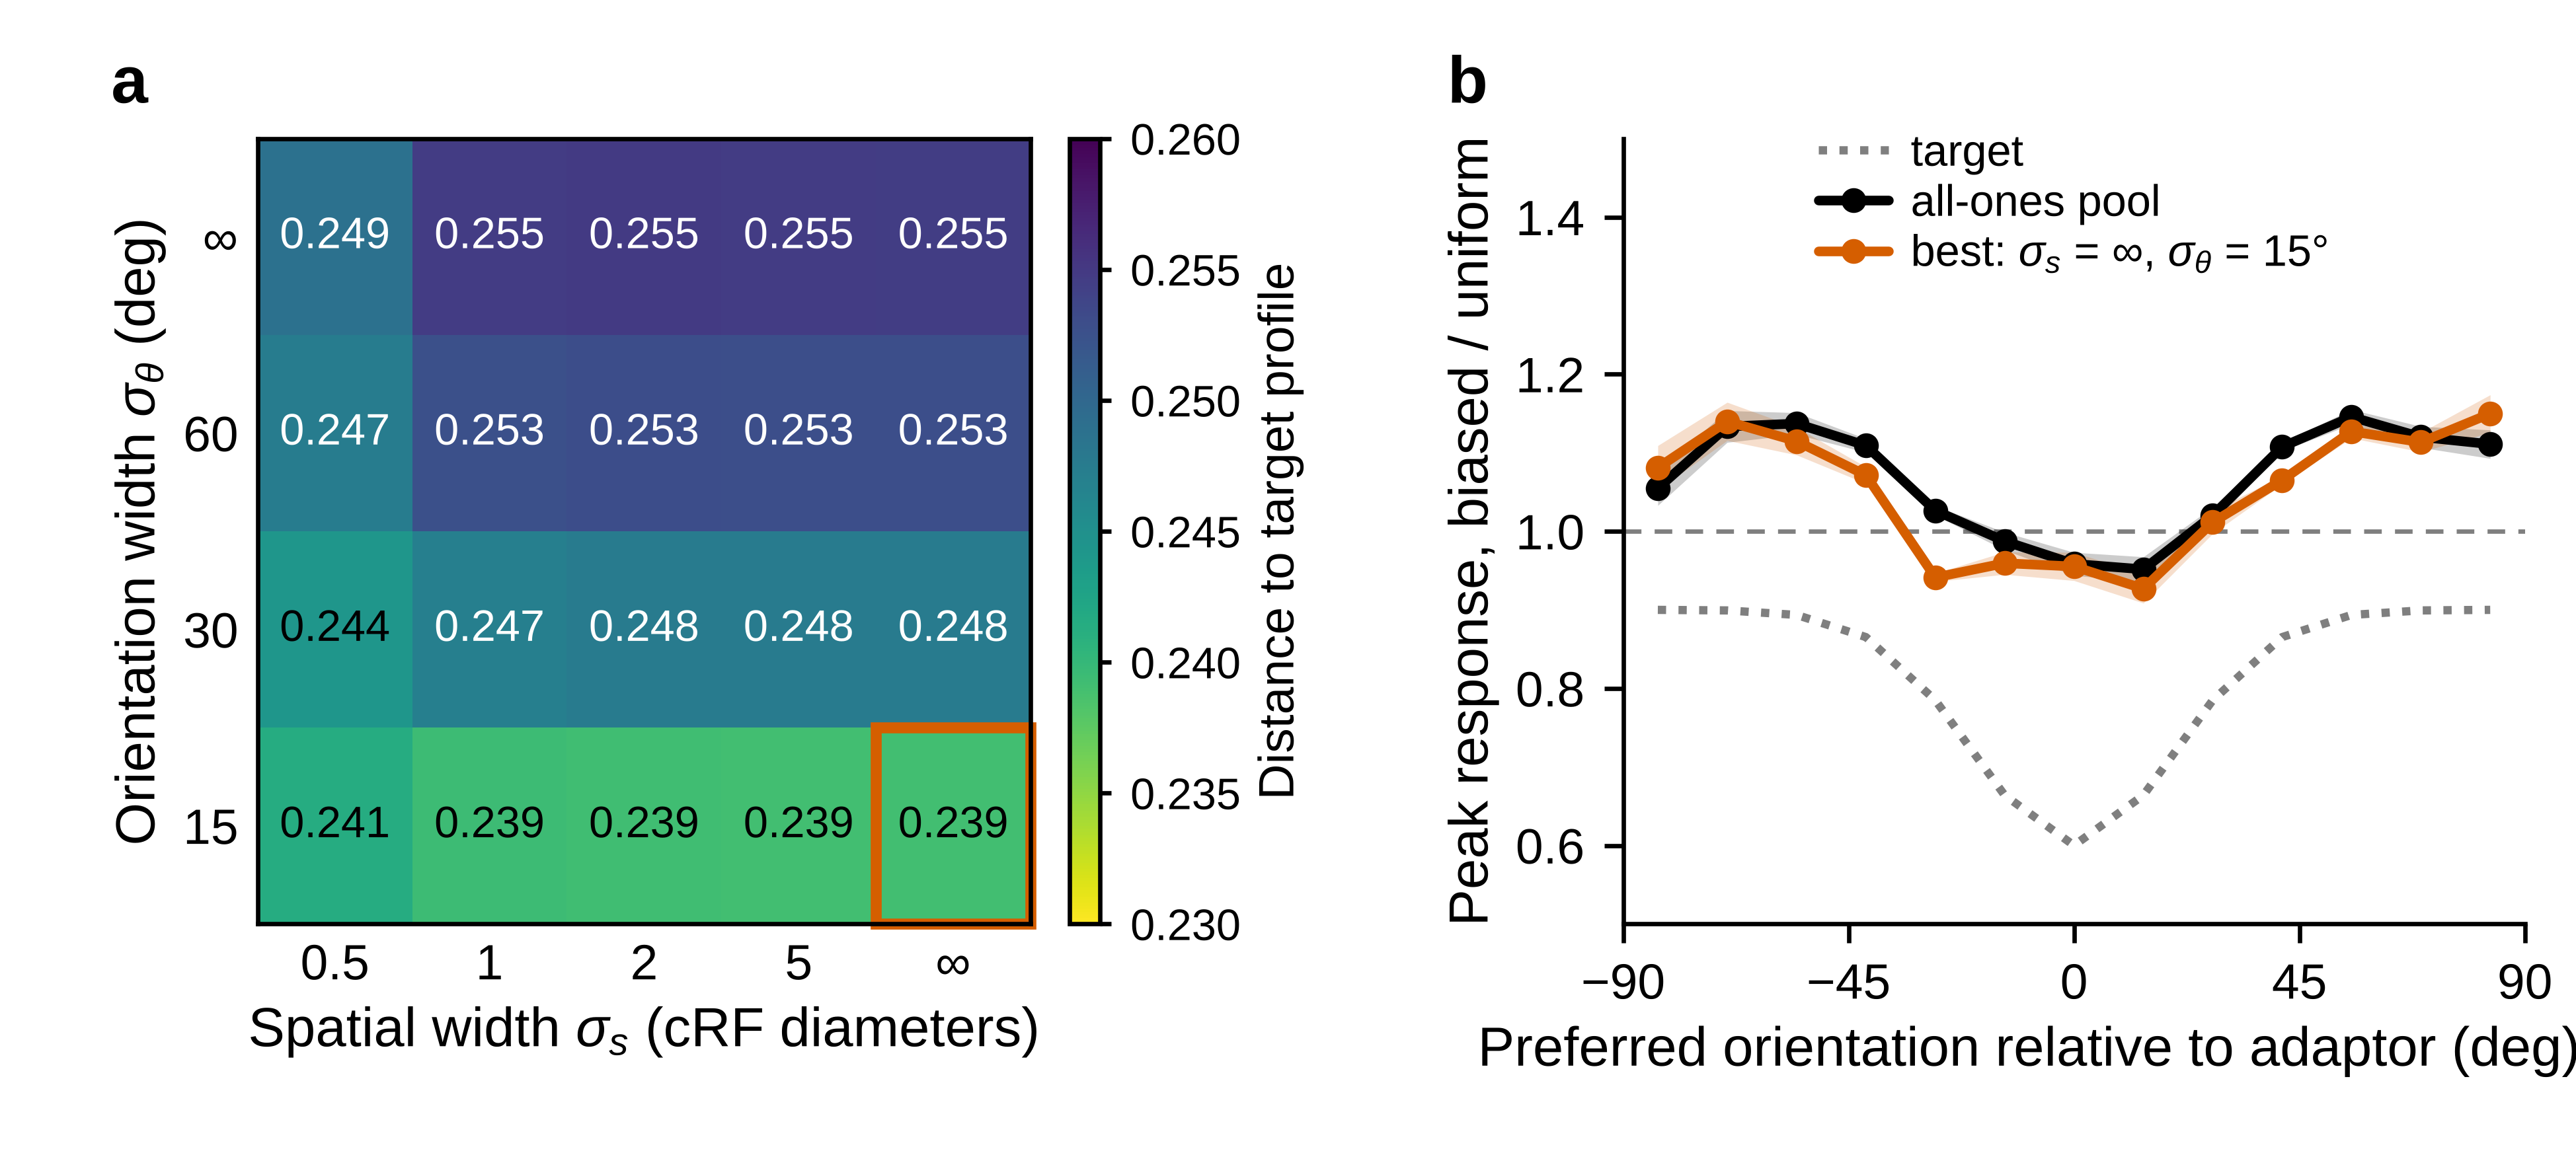
\includegraphics[width=165mm]{FigS7_normalization_widths.png}
\caption{\textbf{Effect of the widths of the normalization pool.} Small adaptors, frozen-gain readout, no noise. \textbf{a}, Distance between the simulated and target profiles for each spatial width $\sigma_s$ and orientation width $\sigma_\theta$ ($\infty$, flat). The top right cell is the all-ones pool; the outlined cell is closest to the target. \textbf{b}, Suppression profiles (mean $\pm$ s.e.m.) for the all-ones pool and the closest pool; dotted, target.}
\label{fig:widths}
\end{figure}

\blurb{Supplementary Fig.~\ref{fig:widths}.} We repeated the adaptation experiment for 20 combinations of spatial and orientation width. The figure shows how close each came to the target profile. The widths had almost no effect: the distance ranged from 0.239 to 0.255, the ratio far from the adaptor from 1.10 to 1.12, and the ratio at the adaptor from 0.95 to 0.97. Narrow orientation tuning ($\sigma_\theta=15^\circ$) was marginally closer for every spatial width. Simulated steady states deviated from Eqs.~10 and 11 of the main text by up to 91\% of the peak response for the narrowest pools and by at most 8\% for $\sigma_s\ge2$ and $\sigma_\theta\ge60^\circ$, which confirms that the analytic fixed point cannot be used for non-uniform weights.

\begin{figure}[H]
\centering
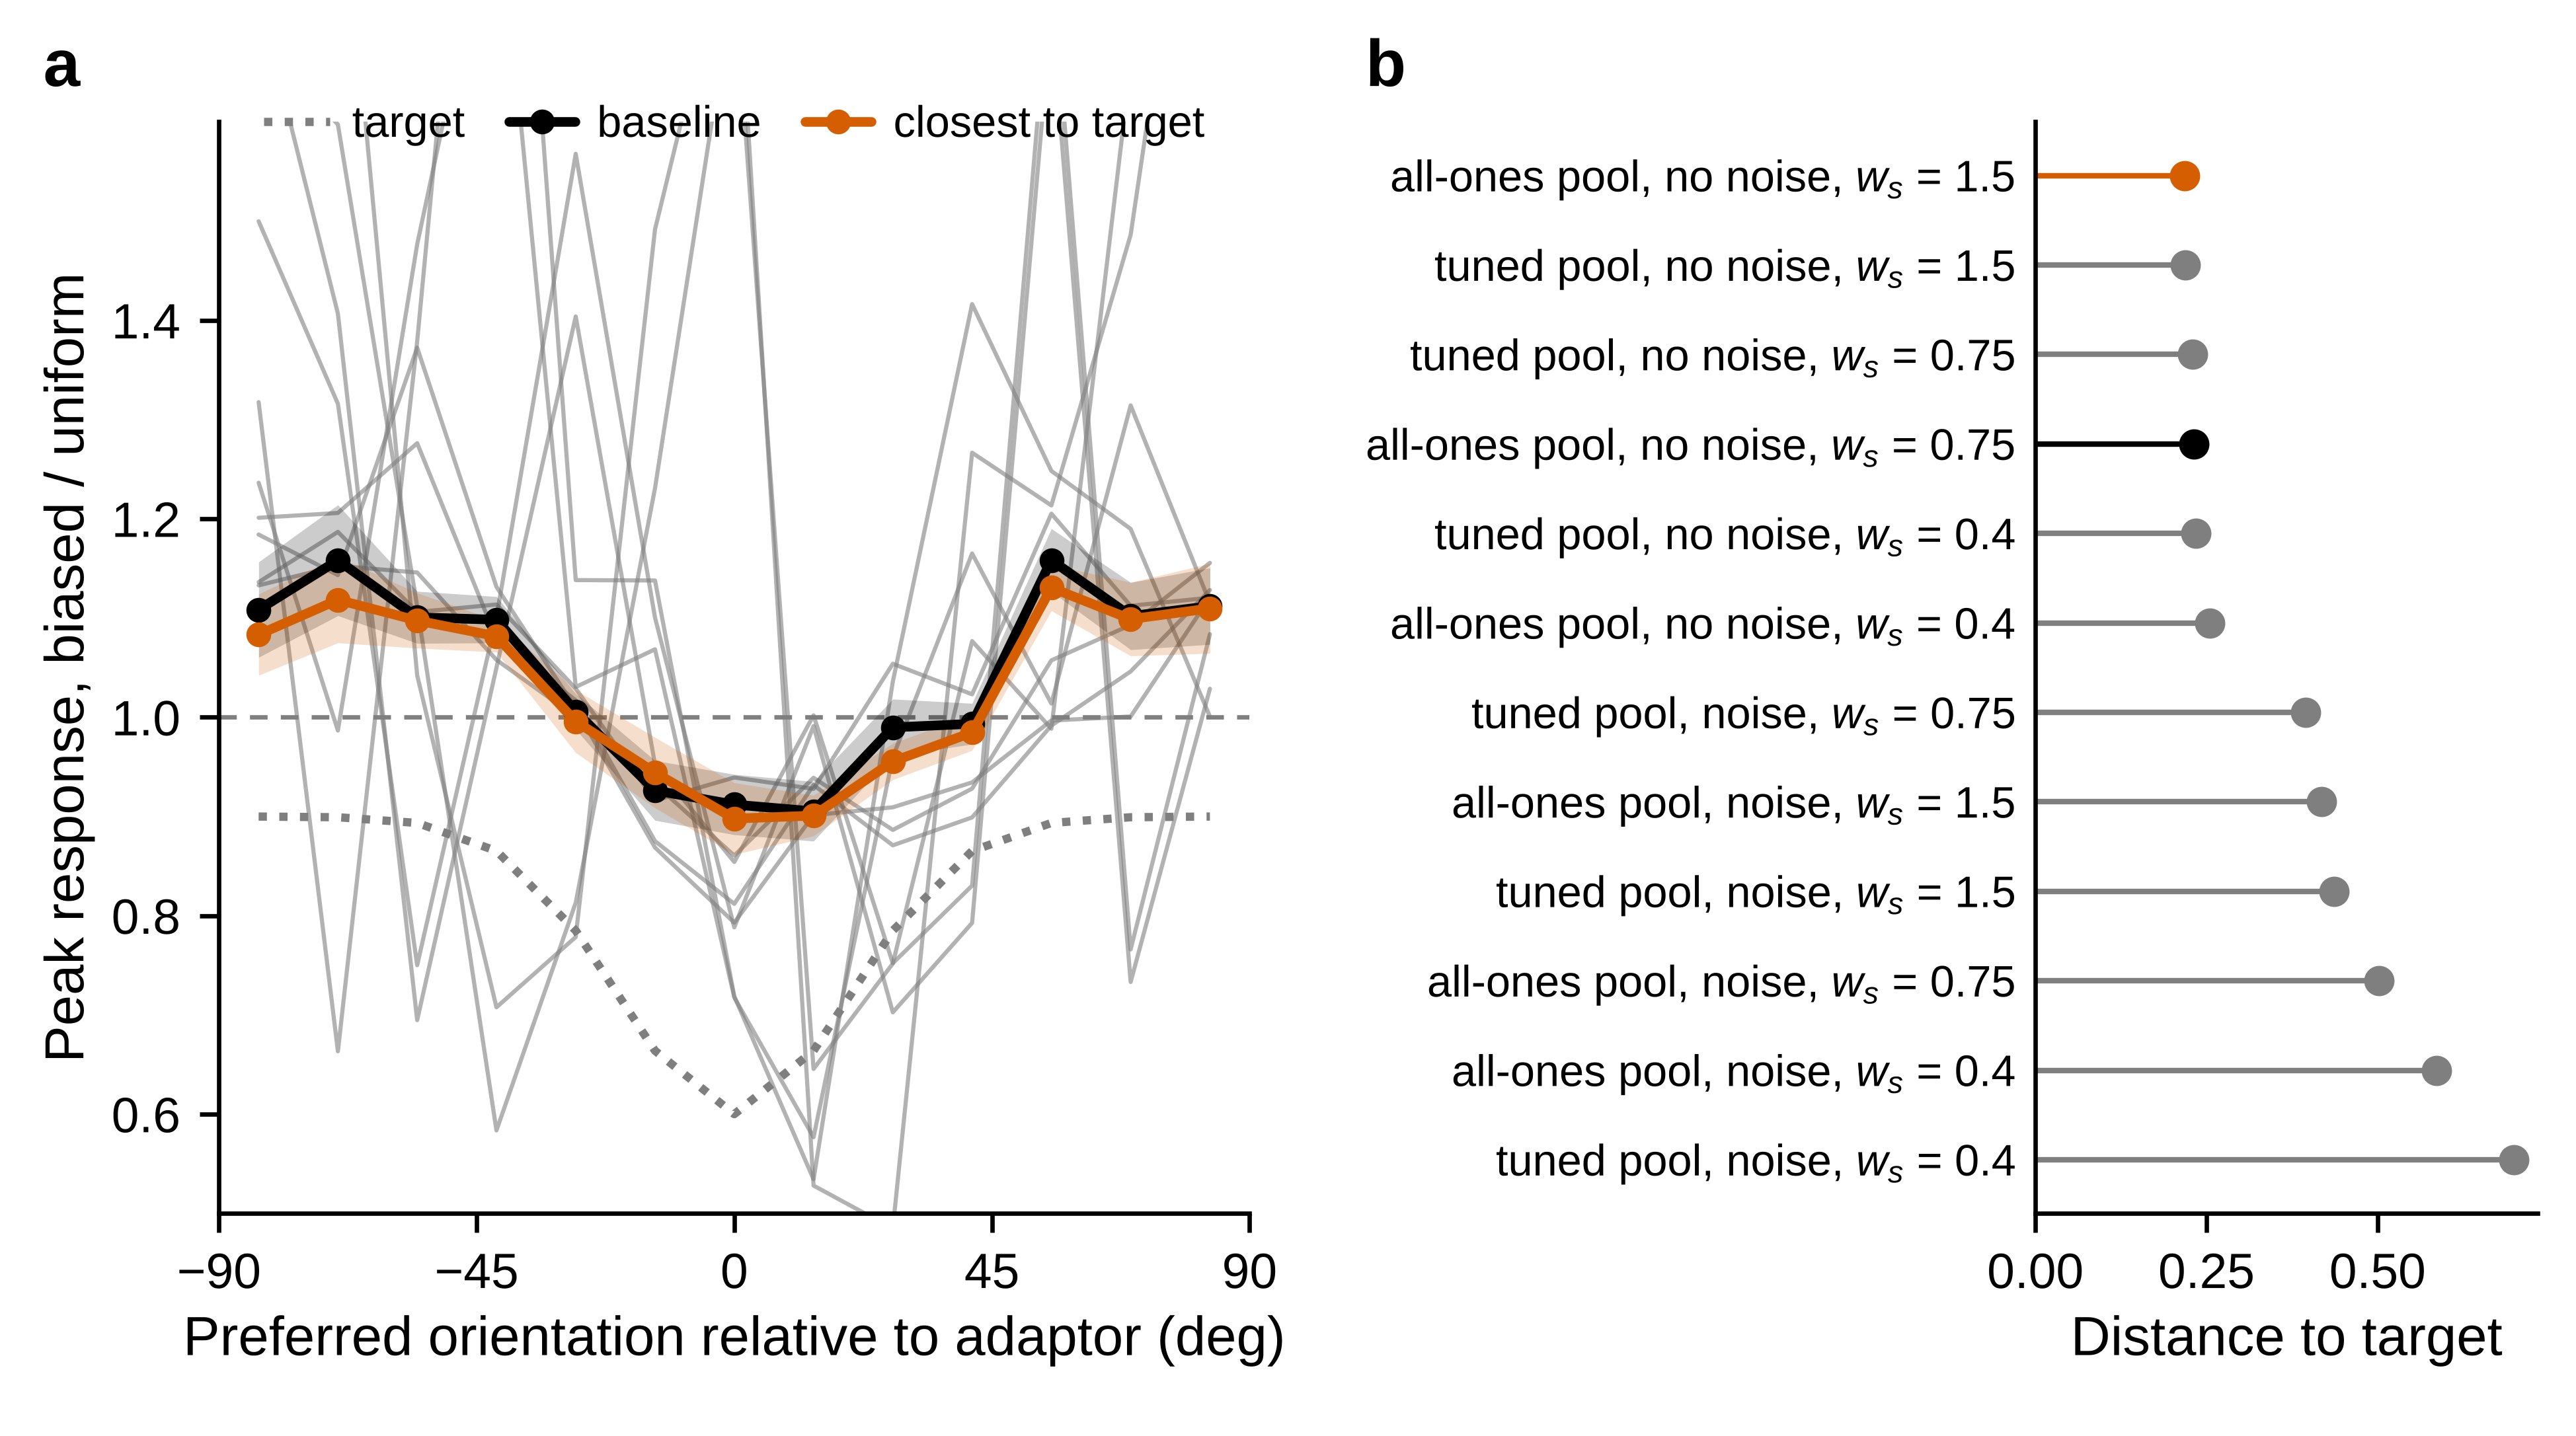
\includegraphics[width=165mm]{FigS8_large_stimuli.png}
\caption{\textbf{Large adaptors: sensitivity analysis.} In-stream readout over the second half of adaptation, 8 random sequences per ensemble. Twelve configurations: all-ones or orientation-tuned normalization pool ($\sigma_s=\infty$, $\sigma_\theta=15^\circ$), with or without Poisson input noise (1000 spikes per second), and three tuning widths $w_s$ of the input to the surround (0.4, 0.75, 1.5~rad; 0.75 is the default). \textbf{a}, Suppression profiles: black, baseline; orange, configuration closest to the target; grey, the others; dotted, target. \textbf{b}, Distance to the target for every configuration.}
\label{fig:large}
\end{figure}

\blurb{Supplementary Fig.~\ref{fig:large}.} We combined the settings that came closest to the target in Supplementary Figs.~\ref{fig:noise} and \ref{fig:widths} and varied the orientation tuning of the surround, for large adaptors. This is a sensitivity analysis over 12 configurations, not a fit. No configuration reproduced the experimental pattern. Without noise the distance ranged from 0.22 to 0.25 (baseline 0.23), the ratio far from the adaptor from 1.11 to 1.15, and the ratio at the adaptor from 0.79 to 0.94. Noise made the in-stream profiles irregular and increased the distance. The feature the model fails to capture is the untuned suppression: responses far from the adaptor were facilitated in every configuration. The suppression at the adaptor was also shallower than the target, and deepened only when the orientation-tuned pool was used.

%=====================================================================
\clearpage
\suppnote{Rectified variance}

We tested whether the gains should follow a rectified measure of variance that grows only when the input current is above its running mean:
\begin{equation}
\tau_g \frac{d\bm{g}}{dt} = \lfloor \bm{c}-\bm{\mu}\rfloor^2 - \bm{\theta}_t^{\text{rect}}, \qquad \bm{\theta}_t^{\text{rect}} = \tfrac12\,\bm{\theta}_t .
\end{equation}
The target is halved because the rectified square of a zero-mean Gaussian variable is half its variance. Note that ``above the mean'' holds for each interneuron, not for each principal neuron: the columns of $\bm{W}_{yv}$ have mixed signs, so $\bm{c}$ can rise above $\bm{\mu}$ when some principal neurons fall below their own means.

A simple case gives an expectation. A neuron that responds with amplitude $A$ on a fraction $p$ of presentations has variance $A^2p(1-p)$ and rectified variance $A^2p(1-p)^2$, so rectification keeps a fraction $1-p$. Neurons tuned to the adaptor ($p\approx\tfrac13$) keep less than rarely driven neurons, which should shift suppression away from the adaptor and toward the orthogonal orientation.

\begin{figure}[H]
\centering
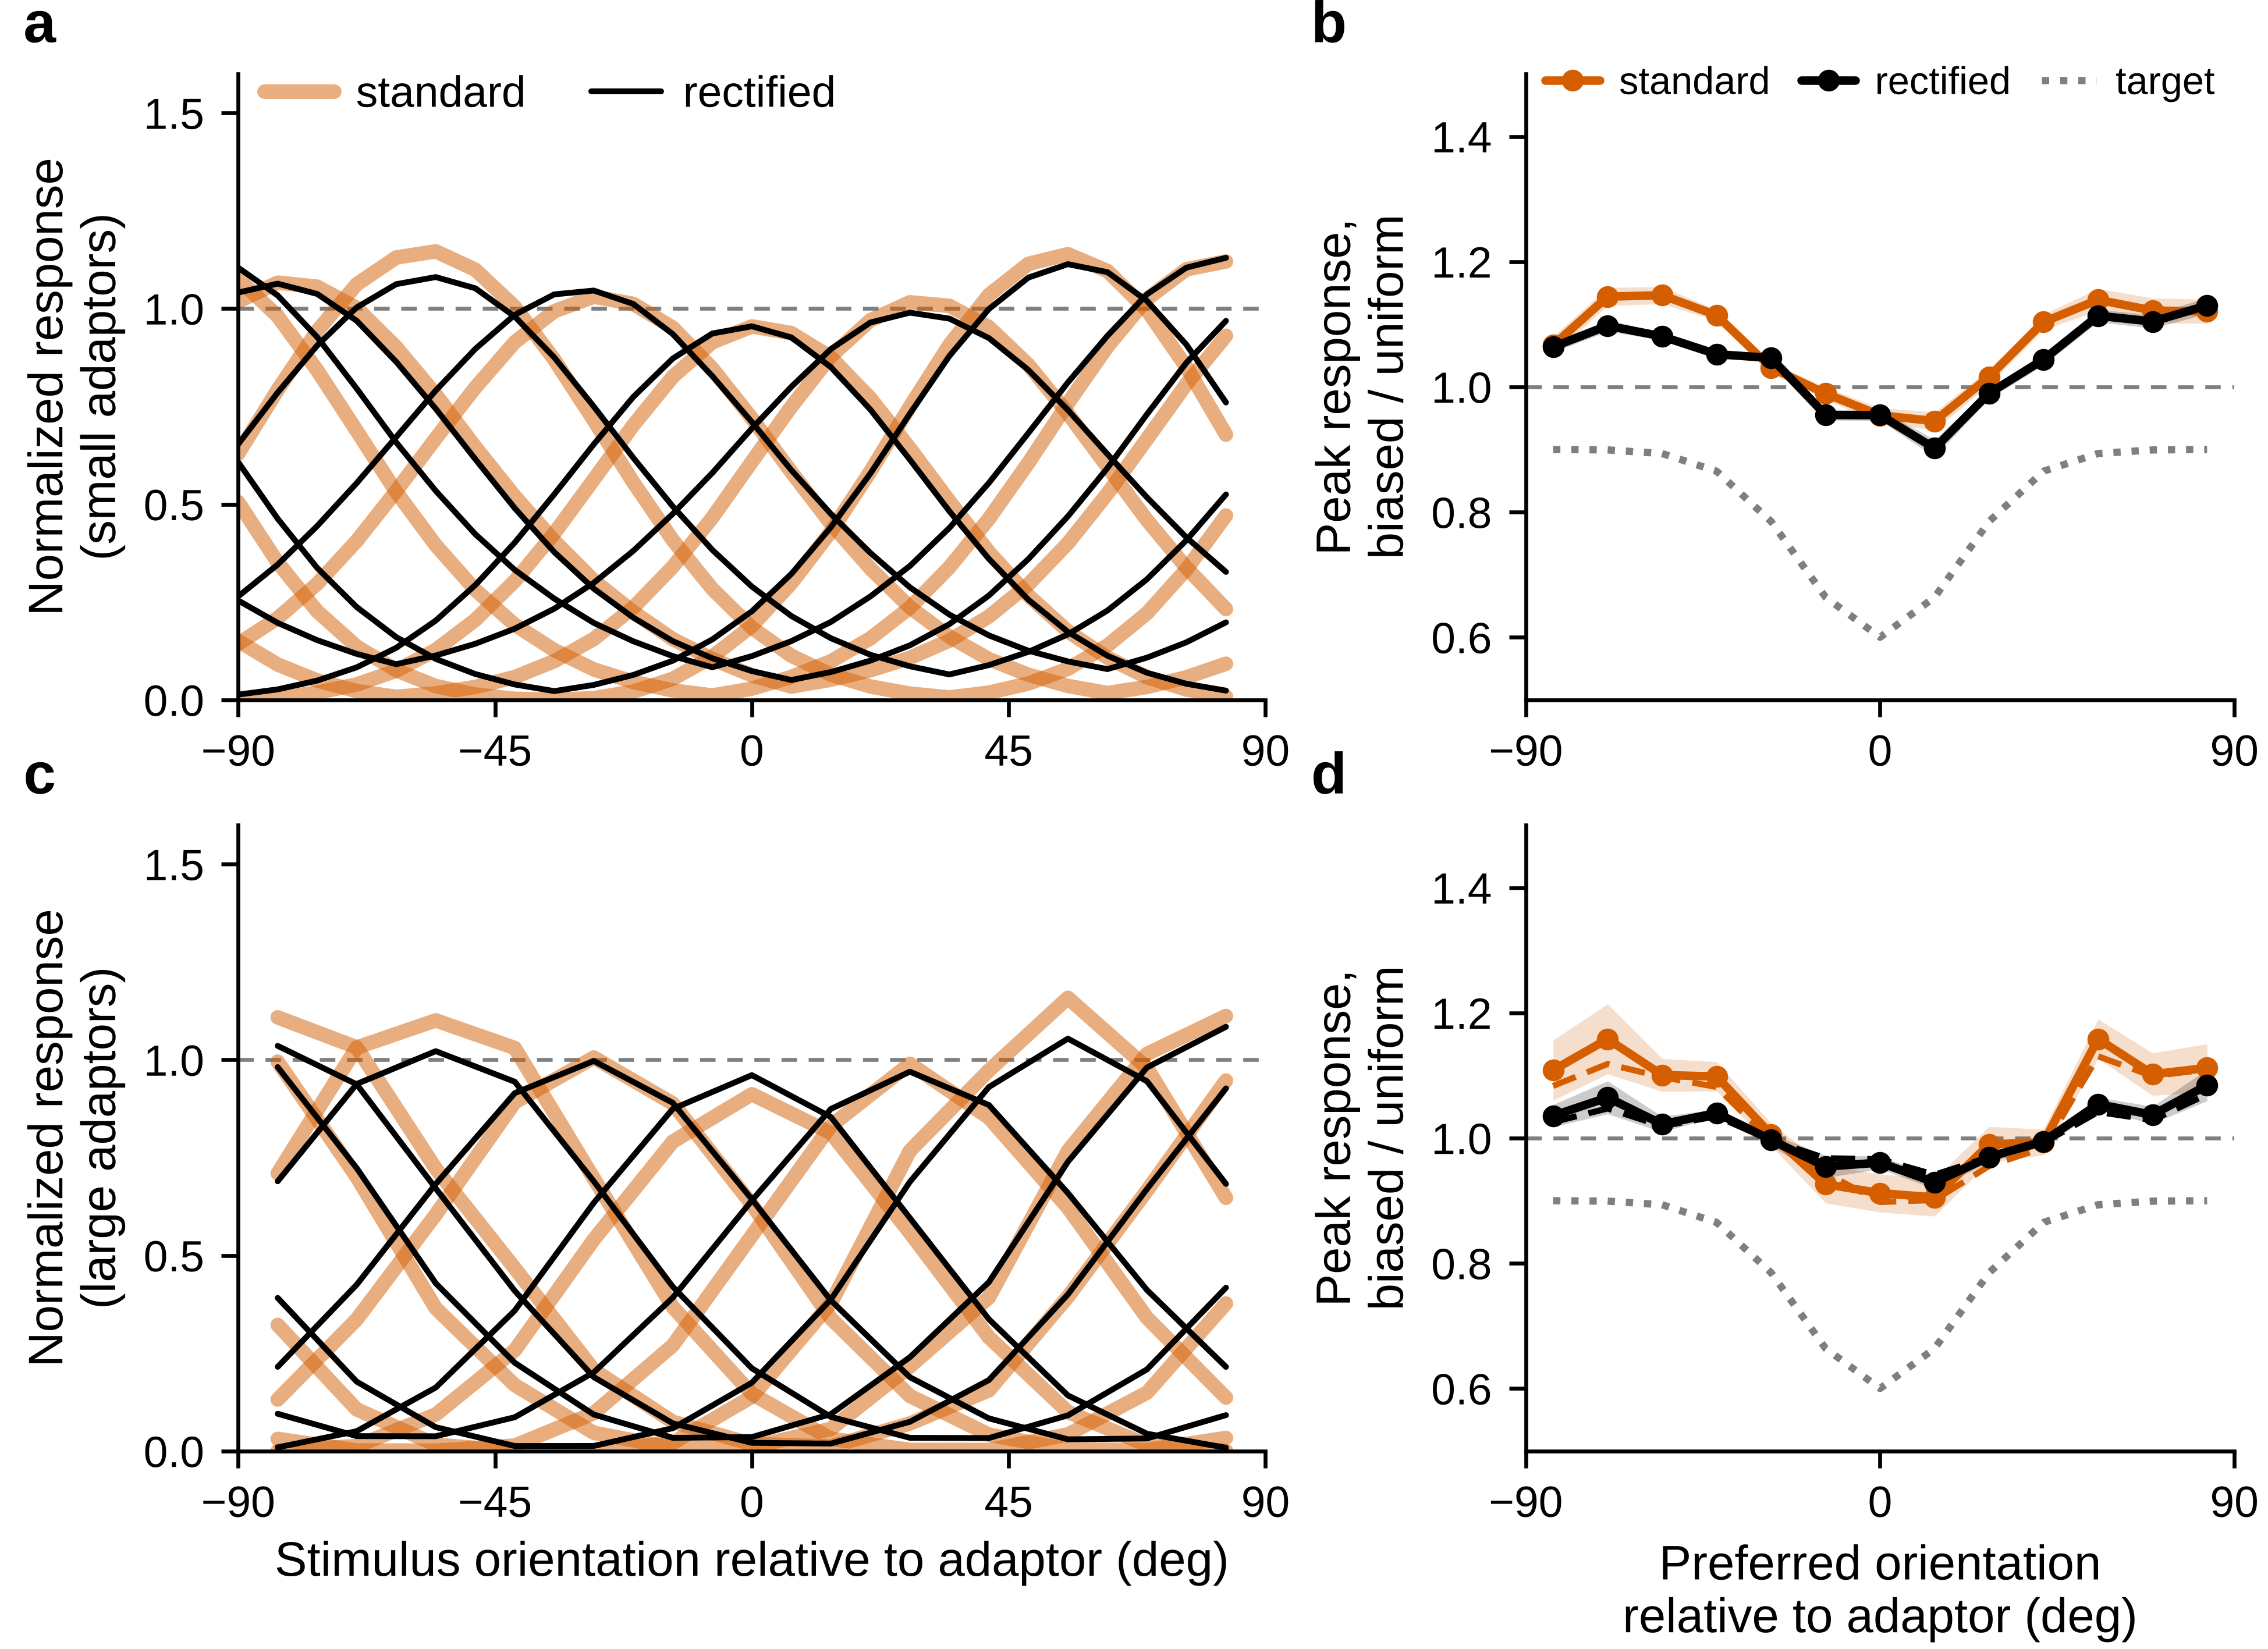
\includegraphics[width=165mm]{FigS9_rectified_variance.png}
\caption{\textbf{Standard versus rectified variance.} Eight random sequences per ensemble. \textbf{a}, Small adaptors, frozen-gain readout: tuning curves of every second cRF neuron after biased adaptation, divided by the neuron's peak after uniform adaptation. \textbf{b}, Suppression profiles (mean $\pm$ s.e.m.); dotted, target. \textbf{c, d}, The same for large adaptors with the in-stream readout. Dashed lines in d, the configuration closest to the target in Supplementary Fig.~\ref{fig:large} (surround tuning width 1.5~rad), which is identical to the baseline for small adaptors.}
\label{fig:rectified}
\end{figure}

\blurb{Supplementary Fig.~\ref{fig:rectified}.} We ran the ensemble experiment with the standard and the rectified gain equation, for small and large adaptors. The figure shows the resulting tuning curves and suppression profiles. Rectification roughly halved the gains even with the halved target (mean gain 0.050 instead of 0.111 for small adaptors, 0.017 instead of 0.050 for large adaptors), so all profiles moved toward one. The distance to the target fell slightly (0.23 instead of 0.26 for small adaptors, 0.21 instead of 0.23 for large adaptors), but only because adaptation was weaker overall: responses far from the adaptor were still facilitated (ratio 1.05--1.10) and the suppression at the adaptor did not deepen (0.96). For large adaptors the profile shifted in the expected direction, with less suppression at the adaptor ($+0.05$) and more at the orthogonal orientation ($-0.07$); for small adaptors the shift was within the error. Rectifying the variance does not bring the profile closer to experiment.

\begin{thebibliography}{9}
\raggedright

\bibitem{tring_power_2023}
Tring, E., Dipoppa, M., Ringach, D.L.: A power law describes the magnitude of adaptation in neural populations of primary visual cortex. Nature Communications \textbf{14}(1), 8366 (2023). https://doi.org/10.1038/s41467-023-43572-w

\bibitem{duong_adaptive_2023-1}
Duong, L.R., Lipshutz, D., Heeger, D.J., Chklovskii, D.B., Simoncelli, E.P.: Adaptive whitening in neural populations with gain-modulating interneurons. arXiv:2301.11955 [q-bio] (2023). https://doi.org/10.48550/arXiv.2301.11955

\bibitem{benucci_adaptation_2013}
Benucci, A., Saleem, A.B., Carandini, M.: Adaptation maintains population homeostasis in primary visual cortex. Nature Neuroscience \textbf{16}(6), 724--729 (2013). https://doi.org/10.1038/nn.3382

\end{thebibliography}

\end{document}
